\chapter{The Derivative}
%Begin Section 1.1
\section{Introduction}
Calculus can be thought of as the analysis of curved shapes.\footnote{It is more
than that, of course, but that definition puts us in good company:
the first European textbook on calculus, written by the French mathematician
Guillaume de l'H\^{o}pital in 1696, was titled \emph{Analyse des Infiniment
Petits pour l'Intelligence des Lignes Courbes} (which translates as
\emph{Analysis of the Infinitely Small for Understanding Curved Lines}). That
book (in French) can be obtained freely in electronic form at
\url{https://archive.org}}
Its development grew out of attempts to solve physical problems.
For example, suppose that an object at rest 100 ft above the ground is dropped.
Ignoring air resistance and wind, the object will fall straight down until it
hits the ground (see Figure \ref{fig:fall}(a)). As will be proved later,
$t$ seconds after being dropped the object will be
$s = s(t) = -16t^2 + 100$ ft above the ground. The object will thus hit
the ground after 2.5 seconds (when $s = 0$). While the object's \emph{path} is a
straight line, the graph of its position $s$ above the ground as a function of
time $t$ is curved, part of a parabola (see Figure \ref{fig:fall}(b)).

\begin{figure}[ht]
 \centering
 \subfloat[][ Path of the object]{
 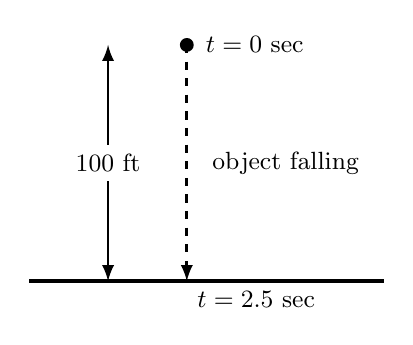
\begin{tikzpicture}[>=latex,every node/.style={font=\small}]
  \draw [line width=1pt,<->] (-1,0) -- (-1,3)
   node[midway,fill=white] {$100$ ft};
  \draw [dashed,line width=1pt,->] (0,3) -- (0,0)
   node [right,pos=0.0] {$~t=0$ sec} node [below right,pos=1.0] {$t=2.5$ sec};
  \draw [line width=1.2pt] (-2,0) -- (2.5,0);
  \fill (0,3) circle (2.5pt);
  \node [right] at (0.2,1.5) {object falling};
 \end{tikzpicture}}
 \qquad\qquad
 \subfloat[][ Position $s$ as a function of time $t$]{
 \begin{tikzpicture}[>=latex,every node/.style={font=\small}]
  \node[below left] at (0,0) {$0$};
  \draw [linecolor,line width=1.5pt] (0,3) parabola (2.5,0);
  \node[right] at (1.8,1.85) {$s=-16t^2 + 100$};
  \draw [<->,black!60,line width=1pt] (0,3.8) node[above] {$s$}
   |- (5.5,0) node[right] {$t$};
  \fill (0,3) circle (2.5pt);
  \fill (2.5,0) circle (2.5pt);
  \node [left] at (0,3) {$100$};
  \node [below] at (2.5,0) {$2.5$};
 \end{tikzpicture}}
 \caption[]{\quad An object dropped from 100 ft above the ground}
 \label{fig:fall}
\end{figure}

How fast is the object moving before it hits the ground? This is where
calculus comes in. The solution, presented now, will motivate much of this
chapter.\index{straight line motion}

First, the object travels 100 ft in 2.5 seconds, so its \textbf{average speed}
in that time is\index{speed}
\begin{displaymath}
 \frac{\text{distance traveled}}{\text{time elapsed}} ~=~
 \frac{100 \text{ ft}}{2.5 \text{ seconds}} ~=~ 40 \text{ ft/s,}
\end{displaymath}
and its \textbf{average velocity}\index{velocity!average} in that time is
\begin{displaymath}
 \frac{\text{change in position}}{\text{change in time}} ~=~
 \frac{\text{final position} ~-~ \text{initial position}}
 {\text{end time} ~-~ \text{start time}} ~=~
 \frac{0 \text{ ft} ~-~ 100 \text{ ft}}{2.5 \text{ sec} ~-~ 0 \text{ sec}} ~=~
 -40 \text{ ft/s.}
\end{displaymath}
Unlike speed, velocity takes direction into account. Thus, the object's downward
motion means it has negative velocity. Positive velocity implies upward motion.

\par Using the idea of average velocity over an interval of time, there is a
natural way to define the object's
\textbf{instantaneous velocity}\index{velocity!instantaneous}\index{velocity}
at a particular \emph{instant} of time $t$:
\begin{enumerate}
 \item Find the average velocity over an interval of time.
 \item Let the interval become smaller and smaller indefinitely, shrinking
  to a point $t$. If the average velocity over that smaller and smaller
  interval approaches some value, call that value the instantaneous velocity
  at time $t$.
\end{enumerate}
Figure \ref{fig:instvel} below shows how to choose the interval: for any
time $t$ between 0 and 2.5, use the interval $\ival{t}{t+\Delta t}$, where
$\Delta t$ (pronounced ``delta t'') is a small positive number. So $\Delta t$
is the change in time over the interval; denote by $\Delta s$ the change in the
position $s$ over that interval.

\begin{figure}[ht]
 \begin{center}
 \begin{tikzpicture}[>=latex,every node/.style={font=\small}]
  \draw [linecolor,line width=1.5pt] (0,4) parabola (5,0);
  \draw[dotted] (2,1.44) -- (2,0);
  \draw[dotted] (4,1.44) -- (4,0);
  \draw[dotted] (2,1.44) -- (0,1.44);
  \draw[dotted] (2,3.36) -- (0,3.36);
  \draw [<->,black!60,line width=1pt,anchor=base] (0,4.8) node[above]
   {$s$} |- (7.5,0) node[right] {$t$}
   node[black,shift={(0,-0.4)}] at (2,0) {$t$}
   node[black,shift={(0,-0.4)}] at (4,0) {$t + \Delta t$}
   node[black,shift={(0,-0.4)}] at (5,0) {$2.5$};
  \fill (0,4) circle (2.5pt);
  \fill (5,0) circle (2.5pt);
  \node[below left] at (0,0) {$0$};
  \node [left] at (0,4) {$100$};
  \fill (2,3.36) circle (2.5pt);
  \fill (4,1.44) circle (2.5pt);
  \draw[dashed] (2,3.36) -- (4,1.44) -- (2,1.44) node[midway,below] {$\Delta t$}
   -- (2,3.36) node[midway,left] {$\Delta s$};
  \draw (2.3,1.44) -- ++(0,0.3) -- ++(-0.3,0);
  \node [left] at (0,1.44) {$s(t + \Delta t)$};
  \node [left] at (0,3.36) {$s(t)$};
  \node [right] at (4,2.6) {average velocity $= \dfrac{\Delta s}{\Delta t} =
  \dfrac{s(t + \Delta t) ~-~ s(t)}{\Delta t}$};
 \end{tikzpicture}\vspace{-4mm}
 \end{center}
 \caption[]{\quad Average velocity $\frac{\Delta s}{\Delta t}$ over the interval
  $\ival{t}{t+\Delta t}$}
 \label{fig:instvel}
\end{figure}

The average velocity of the object over the interval $\ival{t}{t+\Delta t}$ is
$\frac{\Delta s}{\Delta t}$, so since $s(t) = -16t^2 + 100$:

\begin{align*}
 \dfrac{\Delta s}{\Delta t} ~~&=~~ \dfrac{s(t + \Delta t) ~-~ s(t)}
  {\Delta t}\\[8pt]
  &=~~ \dfrac{-16(t+\Delta t)^2 ~+~ 100 ~-~ (-16t^2 ~+~ 100)}{\Delta t}\\[8pt]
  &=~~ \dfrac{-16t^2 ~-~ 32t\Delta t ~-~ 16(\Delta t)^2 ~+~ 100 ~+~ 16t^2
   ~-~ 100}{\Delta t}\\[8pt]
  &=~~ \dfrac{-32t\Delta t ~-~ 16(\Delta t)^2}{\Delta t}
   ~~=~~ \dfrac{\cancel{\Delta t} \,(-32t ~-~ 16\Delta t)}
          {\cancel{\Delta t}}\\[6pt]
  &=~~ -32t ~-~ 16\Delta t ~,
\end{align*}
Now let the interval $\ival{t}{t+\Delta t}$ get smaller and
smaller indefinitely---that is, let $\Delta t$ get closer and closer to 0.
Then the average velocity $\frac{\Delta s}{\Delta t} = -32t - 16\Delta t\,$
gets closer and closer to $-32t - 0 = -32t$. Thus, \emph{the object has
instantaneous velocity $-32t$ at time $t$}. This calculation can be
interpreted as taking the \textbf{limit}\index{limit} of
$\frac{\Delta s}{\Delta t}\,$ \emph{as} $\Delta t\,$ \emph{approaches} $0$,
written as follows:
\begin{align*}
 \text{instantaneous velocity at $t$} ~~&=~~
  \text{limit of average velocity over $\ival{t}{t+\Delta t}$
  as $\Delta t$ approaches to 0}\\[6pt]
  &=~~ \lim_{\Delta t \to 0} ~\frac{\Delta s}{\Delta t}\\[8pt]
  &=~~ \lim_{\Delta t \to 0} ~(-32t ~-~ 16\Delta t)\\[6pt]
  &=~~ -32t - 16(0)\\[6pt]
  &=~~ -32t
\end{align*}

Notice that $\Delta t$ is not replaced by $0$ in the
ratio $\frac{\Delta s}{\Delta t}$ until \emph{after} doing as much cancellation
as possible. Notice also that the instantaneous velocity of the object
varies with $t$, as it should (why?). In particular, at the instant when the
object hits the ground at time $t = 2.5$ sec, the instantaneous velocity is
$-32(2.5) = -80$ ft/s.

If this makes sense so far, then you understand the crux of the idea of what a
limit is and how to calculate a limit. The instantaneous velocity $v(t) = -32t$
is called the \textbf{derivative} of the position function $s(t) =-16t^2 + 100$.
Calculating derivatives, analyzing their properties, and using them to solve
various problems are part of \emph{differential calculus}.\index{derivative}

What does this have to do with curved shapes? Instantaneous velocity is a
special case of an \textbf{instantaneous rate of change}\index{instantaneous
rate of change} of a function; in this case the instantaneous rate of change of
the position (height above the ground) of the object. Similar to how the rate
of change of a line is its slope, the instantaneous rate of change of a general
curve represents the \textbf{slope of the curve}. For example, the parabola
$s(t) = -16t^2 + 100$ has slope $-32t$ for all $t$. Note that the slope of this
curve varies (as a function of $t$), unlike the slope of a straight line.

Finding the area inside curved regions is another type of problem that calculus
can solve. The basic idea is to use simpler regions---rectangles---whose areas
are known, then use those to approximate the area inside the curved
region. One such method is to draw more and more rectangles of diminishing
widths \emph{inside} the curved region,\footnote{It will be
shown later (in Chapter 5) that the rectangles do not have to be completely
inside the region.} so that the sums of their areas approach the area of the
curved region. Figure \ref{fig:area} shows an example with four
rectangles to approximate the area under a curve $y=f(x)$ over an interval
$\ival{a}{b}$ on which $f(x) \ge 0$.

\begin{figure}[ht]
 \begin{center}
  \begin{tikzpicture}[>=latex,every node/.style={font=\small}]
   \fill [fill=fillcolor] (4.2,1) to[out=140,in=-10] (3,1.5)
    to[out=180,in=0] (2,1) to[out=180,in=-45] (1,1.5) -- (1,0) -- (4.2,0) --
    (4.2,1);
   \draw[line width=1pt] (1,0) -- (1,1.5);
   \draw[line width=1pt] (4.2,0) -- (4.2,1);
   \draw [linecolor,line width=1.5pt] (4.2,1) to[out=140,in=-10] (3,1.5)
    to[out=180,in=0] (2,1) to[out=180,in=-45] (1,1.5);
   \node [above] at (2.5,1.5) {$y = f(x)$};
   \draw [dashed] (1.5,0) -- (1.5,1.125) -- (1,1.125);
   \draw [dashed] (1.5,1) -- (2.5,1);
   \draw [dashed] (2.5,0) -- (2.5,1.26) -- (3.85,1.26) -- (3.85,0);
   \draw [dashed] (3.85,1) -- (4.2,1);
   \draw[<->,black!60,line width=1pt,anchor=base] (0,2.3) node[above] {$y$} |-
    (5,0) node[right] {$x$} node[black,shift={(0,-0.4)}] at (1,0) {$a$}
    node[black,shift={(0,-0.4)}] at (4.2,0) {$b$};
   \fill (1,1.5) circle (2.5pt);
   \fill (4.2,1) circle (2.5pt);
  \end{tikzpicture}\vspace{-6mm}
 \end{center}
 \caption[]{\quad The area of a curved region}
 \label{fig:area}
\end{figure}

The limit of these sums of rectangular areas is called an \textbf{integral}.
The study and application of integrals are part of
\emph{integral calculus}.\index{integral} Perhaps the most remarkable result in
calculus is that there is a connection between derivatives and integrals---the
\emph{Fundamental Theorem of Calculus}, discovered
in the 17\textsuperscript{th} century, independently, by the two men who
invented calculus as we know it: English physicist, astronomer and
mathematician Isaac Newton (1642-1727) and German mathematician and philosopher
Gottfried Wilhelm von Leibniz (1646-1716).

Calculus makes extensive use of \emph{infinite sequences and
series}\index{sequence}\index{series}\index{infinite series}. An
\textbf{infinite series} is just a sum of an infinite number of terms. For
example, it will be shown later in the text that
\begin{equation}\label{eqn:piseries}
 \frac{\pi}{4} ~~=~~ 1 ~-~ \frac{1}{3} ~+~ \frac{1}{5} ~-~ \frac{1}{7} ~+~
 \frac{1}{9} ~-~ \cdots ~,
\end{equation}
where the sum on the right involves an infinite number of terms. A \textbf{power
series}\index{power series} is a particular type of infinite series applied to
functions; it can be thought of as a polynomial of infinite degree. For example,
the trigonometric function $\sin\;x$ does not appear to be a polynomial. But it
turns out that $\sin\;x$ has a power series representation as
\begin{equation}\label{eqn:sinseries}
 \sin\,x ~~=~~ x ~-~ \frac{x^3}{3!} ~+~ \frac{x^5}{5!} ~-~ \frac{x^7}{7!} ~+~
 \frac{x^9}{9!} ~-~ \cdots ~,
\end{equation}
where again the sum continues infinitely, and the formula holds for all $x$ (in
radians).

The idea of replacing a function by its power series played an important role
throughout the development of calculus, and is a powerful technique in many
applications.

All the functions in this text will be functions of a single real
variable---that is, the values that the variable can take are real
numbers. Below is some standard notation for commonly-used sets
of numbers:\index{real numbers}\index{$\mathbb{R}$}\index{rational
numbers}\index{$\mathbb{Q}$}\index{integers}
\index{$\mathbb{I}$}\index{natural numbers}\index{$\mathbb{N}$}

\begin{align*}
 \Naturals ~~&=~~ \text{the set of all \textbf{natural} numbers, i.e. the set of
  nonnegative integers: } 0, 1, 2, 3, 4, \ldots\\[6pt]
 \Integers ~~&=~~ \text{the set of all integers: } 0, \pm 1, \pm 2, \pm 3,
  \pm 4, \ldots\\[6pt]
 \Rationals ~~&=~~ \text{the set of all \textbf{rational} numbers $\frac{m}{n}$,
  where $m$ and $n$ are integers, with $n \ne 0$}\\[6pt]
 \Reals ~~&=~~ \text{the set of all real numbers}
\end{align*}
Note that $\Naturals ~~\subset~~ \Integers ~~\subset~~ \Rationals ~~\subset~~
\Reals$.

The set of real numbers consists of the rational numbers together with numbers
that are not rational, called \textbf{irrational numbers}.\index{irrational
numbers} For example, $\sqrt{2}$ is irrational. That is, 2 is not the square of
a rational number. In fact, if the square of a rational number $q$ were an
integer, then $q$ itself would have to be an integer: write $q$ as $m/n$, where
$m$ and $n$ are positive integers with no common positive integer divisors other
than 1. Since $q^2 = m^2/n^2$ simply duplicates the integer divisors of $m$ and
$n$, then $q^2$ can be an integer only if $n=1$, i.e. $q$ is an integer. Clearly
2 is not the square of an integer, and thus it cannot be the square of a
rational number. This argument also shows that $\sqrt{3}$, $\sqrt{5}$,
$\sqrt{6}$, $\sqrt{7}$, $\sqrt{8}$, $\sqrt{10}$, and so on, are
irrational.\footnote{This argument is due to the British philosopher Bertrand
Russell (1872-1970). For an alternative proof that $\sqrt{2}$ is irrational, see
pp. 97-98 in \textsc{Gelfand, I.M. and A. Shen}, \emph{Algebra}, Boston:
Birkh\"{a}user, 1993.}

It turns out that there are far more irrational numbers--and hence real
numbers---than rational numbers. In fact, whereas the rational numbers can be
listed in a sequence (i.e. first, second, third, etc.), the set of real numbers
cannot.\footnote{For a proof see Ch.1 in \textsc{Kamke, E.}, \emph{Theory of
Sets}, New York: Dover Publications, Inc., 1950.} For example, in the closed
interval $\ival{0}{1}$ there is no ``next'' real number after the number $0$.
Thus, some infinite sets are larger than others---$\Reals$ is larger than
$\Rationals$. Intervals such as $\ival{0}{1}$
or $\Reals$ itself are examples of a \emph{continuum} of objects, i.e. no
gaps exist.\footnote{For a study of the structure of the real number system, see
\textsc{Burrill, C.W.}, \emph{Foundations of Real Numbers}, New York:
McGraw-Hill Book Company, 1967.}
A famous unsolved problem in mathematics---the \emph{Continuum Hypothesis}---is
whether an infinite set exists that is larger in size than $\Rationals$ but
smaller than $\Reals$.

\emph{Infinity} is an important notion in calculus. Whether it is the idea
of \emph{infinitely large} or \emph{infinitesimally small}, calculus attempts to
give the idea some mathematical meaning (typically by way of
limits).\footnote{Not everyone agrees that calculus does this satisfactorily.
For example, for an alternative development of basically the same material
in ``standard'' calculus but without the use of limits---called
\emph{infinitesimal analysis}---see \textsc{Keisler, H.J.}, \emph{Elementary
Calculus: An Infinitesimal Approach}, Boston: Prindle, Weber \& Schmidt, 1976.}
The mathematical use of infinity has been a subject of philosophical
debate.\footnote{For example, see the essays by L. E. J. Brouwer, Hermann
Weyl and David Hilbert in \textsc{Heijenoort, J. van}, \emph{From Frege to
G{\"o}del: A Source Book in Mathematical Logic, 1879-1931}, Cambridge, MA:
Harvard University Press, 1967.}

Though several centuries old, calculus was the beginning of \emph{modern}
mathematics. \emph{Classical} mathematics (e.g. algebra, geometry,
trigonometry)---whose origins date back to the ancient Babylonians, Egyptians,
and Greeks---was concerned mostly with the study of \emph{static} quantities.
Calculus produced a way to analyze \emph{dynamic} (i.e. changing) quantities.
The period from the 17\textsuperscript{th} through the 19\textsuperscript{th}
century also saw revolutionary advances in physics, chemistry, biology and other
sciences. The birth of calculus was one part of that qualitative leap.
\newpage
\startexercises\label{sec1dot1}
{\small
\probs{A}
\par\noindent For Exercises 1-4, suppose that an object moves in a straight line
such that its position $s$ after time $t$ is the given function $s=s(t)$. Find
the instantaneous velocity of the object at a general time $t \ge 0$.
You should mimic the earlier example for the instantaneous velocity when
$s = -16t^2 + 100$.
\begin{enumerate}[\bfseries 1.]
 \begin{multicols}{4}
  \item $s = t^2$
  \item $s = 9.8t^2$
  \item $s = -16t^2 + 2t$
  \item $s = t^3$
 \end{multicols}
 \item By equation (\ref{eqn:piseries}), $\pi ~=~ 4\,\left(1 ~-~ \frac{1}{3} ~+~
  \frac{1}{5} ~-~ \frac{1}{7} ~+~ \frac{1}{9} ~-~ \cdots ~\right)$, where the
  $n^{th}$ term in the sum inside the parentheses is $\frac{(-1)^{n+1}}{2n-1}$
  (starting at $n=1$).\footnote{This, by the way, is a terrible formula
  for calculating $\pi$; getting just the 3.14 part requires 119 terms in the
  sum!} So the first approximation of $\pi$ using this formula is
  $\pi \approx 4\,(1) = 4.0$, and the second approximation is $\pi \approx
  4\,\left(1 - \frac{1}{3}\right) = 8/3 \approx 2.66667$. Continue like this
  until two consecutive approximations have $3$ as the first digit before the
  decimal point. How many terms in the sum did this require? Be careful with
  rounding off in the approximations.
\suspend{enumerate}
\probs{B}
\resume{enumerate}[{[\bfseries 1.]}]
 \item In elementary geometry you learned that the area inside a circle of
  radius $r>0$ is $\pi r^2$ (that formula will be proved later in the text). So
  in particular, let $C$ be a circle of radius $1$. Then the area inside $C$ is
  $\pi$. That area can be approximated by \emph{Eudoxus' method of
  exhaustion}.\index{Eudoxus}\index{method of exhaustion}\footnote{Originally
  due  to another ancient Greek mathematician, Antiphon (ca. 430 \textsc{b.c.})}
  The idea is to inscribe \emph{regular polygons}\index{regular polygon} inside
  the circle, i.e. the vertexes of the polygons touch $C$. Recall from geometry
  that a polygon is regular if its sides are of equal length. By increasing the
  number of sides of the polygons, the areas inside the polygons will approach
  the area ($\pi$) of $C$. This was an early attempt at using what is now
  called a limit.\footnote{The great ancient Greek mathematician, physicist and
  astronomer Archimedes (ca. 287-212 \textsc{b.c.}) used this method, together
  with circumscribed regular polygons, to calculate $\pi$.}

\begin{figure}[ht]
\begin{minipage}[b]{7.5cm}
 \begin{center}
  \begin{tikzpicture}[every node/.style={font=\small}]
   \filldraw [linecolor,fill=fillcolor,line width=1pt] (45:1.5) -- (135:1.5) --
    (225:1.5) -- (315:1.5) -- cycle;
   \draw [line width=1pt] (0,0) circle (1.53);
   \draw [linecolor,dashed] (0,0) -- (45:1.5) node[black,midway,below] {$1$};
   \fill (0,0) circle (2pt);
   \node [left] at (150:1.58) {$C$};
  \end{tikzpicture}\vspace{-5mm}
 \end{center}
 \caption[]{\quad Inscribed square}
 \label{fig:insquare}
\end{minipage}
\begin{minipage}[b]{7.5cm}
 \begin{center}
  \begin{tikzpicture}[every node/.style={font=\small}]
   \filldraw [linecolor,fill=fillcolor,line width=1pt] (0:1.5) -- (60:1.5) --
    (120:1.5) -- (180:1.5) -- (240:1.5) -- (300:1.5) -- cycle;
   \draw [line width=1pt] (0,0) circle (1.53);
   \draw [linecolor,dashed] (0,0) -- (1.5,0) node[black,pos=0.4,above] {$1$};
   \fill (0,0) circle (2pt);
   \node [left] at (150:1.58) {$C$};
  \end{tikzpicture}\vspace{-5mm}
 \end{center}
 \caption[]{\quad Inscribed regular hexagon}
 \label{fig:inhexagon}
\end{minipage}
\end{figure}\vspace{-2mm}

 \begin{enumerate}[\bfseries (a)]
  \item Inscribe a square inside $C$, as in Figure \ref{fig:insquare}. Show that
   the area inside the square is $2$. This is a poor approximation of $\pi =
   3.14159265...$, obviously.
  \item Inscribe a regular hexagon ($6$-sided)
   inside $C$, as in Figure \ref{fig:inhexagon}. Show that the area inside the
   hexagon is $\frac{3\,\sqrt{3}}{2} \approx 2.59807621$. This is a slightly
   better---though still poor---approximation of $\pi$.
  \item Inscribe a regular dodecagon ($12$-sided) inside $C$. Show that the
   area inside the dodecagon is $3$. It thus takes $12$ sides for the
   approximation to get the first digit of $\pi$ correct.
  \item Inscribe a regular $100$-sided polygon inside $C$. Show that the area
   inside this polygon is approximately $3.13952598$. This is getting closer to
   $\pi$.
  \item Show that the general formula for the area inside a regular $n$-sided
   polygon inscribed inside $C$ is $\dfrac{n}{2}\,\sin\,\left(
   \dfrac{360\Degrees} {n}\right)$. \emph{(Hint: The double-angle identity
   $\sin\,2\theta = 2\,\sin\,\theta\;\cos\,\theta$ might help.)}
 \end{enumerate}
\newpage
\suspend{enumerate}
\probs{C}
\resume{enumerate}[{[\bfseries 1.]}]
 \item What is the flaw in the following ``proof'' that $\pi = 4$?:

\parpic[r]{\begin{tikzpicture}[every node/.style={font=\small}]
 \filldraw [linecolor,fill=fillcolor,line width=1pt] (0,0) circle (1.5);
 \draw [linecolor,dashed] (-1.5,0) -- (1.5,0) node[black,midway,above] {$d =1$};
 \draw [black,line width=1pt] (-1.5,1.5) rectangle (1.5,-1.5);
\end{tikzpicture}}
\noindent\textbf{Step 1:} Draw a square around a circle of diameter $d = 1$.
The circumference of the circle is thus $\pi\,d = \pi$, and the perimeter of the
square is 4.\vspace{29mm}

\parpic[r]{\begin{tikzpicture}[every node/.style={font=\small}]
 \draw [black!60,dotted,line width=0.75pt] (-1.5,1.5) rectangle (1.5,-1.5);
 \filldraw [linecolor,fill=fillcolor,line width=1pt] (0,0) circle (1.5);
 \draw [linecolor,dashed] (-1.5,0) -- (1.5,0) node[black,midway,above] {$d =1$};
 \draw [black,line width=1pt] (-1.5,-1.09) -- (-1.5,1.09) -- (-1.09,1.09) --
  (-1.09,1.5) -- (1.09,1.5) -- (1.09,1.09) -- (1.5,1.09) -- (1.5,-1.09) --
  (1.09,-1.09) -- (1.09,-1.5) -- (-1.09,-1.5) -- (-1.09,-1.09) -- cycle;
\end{tikzpicture}}
\noindent\textbf{Step 2:} Remove corners from the square as shown in the picture
on the right, so that four new corners touch the circle. Notice that the
perimeter of the resulting polygon is still 4, since the lengths of the removed
corner pieces are duplicated in the new polygon, so that the lengths of all the
vertical sides add up to 2 while the lengths of all the horizontal sides add up
to 2.\vspace{17mm}

\parpic[r]{\begin{tikzpicture}[every node/.style={font=\small}]
 \draw [black!60,dotted,line width=0.75pt] (-1.09,1.5) rectangle (1.09,-1.5);
 \draw [black!60,dotted,line width=0.75pt] (-1.5,1.09) rectangle (1.5,-1.09);
 \filldraw [linecolor,fill=fillcolor,line width=1pt] (0,0) circle (1.5);
 \draw [linecolor,dashed] (-1.5,0) -- (1.5,0) node[black,midway,above] {$d =1$};
 \draw [black,line width=1pt] (-1.5,-0.84) -- (-1.5,0.84) -- (-1.29,0.84) --
  (-1.29,1.09) -- (-1.09,1.09) -- (-1.09,1.29) -- (-0.84,1.29) -- (-0.84,1.5) --
  (0.84,1.5) -- (0.84,1.29) -- (1.09,1.29) -- (1.09,1.09) -- (1.29,1.09) --
  (1.29,0.84) -- (1.5,0.84) -- (1.5,-0.84) -- (1.29,-0.84) -- (1.29,-1.09) --
  (1.09,-1.09) -- (1.09,-1.29) -- (0.84,-1.29) -- (0.84,-1.5) -- (-0.84,-1.5) --
  (-0.84,-1.29) -- (-1.09,-1.29) -- (-1.09,-1.09) -- (-1.29,-1.09) --
  (-1.29,-0.84) -- cycle;
\end{tikzpicture}}
\noindent\textbf{Step 3:} Remove corners from the polygon in Step 2, as shown in
the picture on the right, so that eight new corners touch the circle. The
perimeter of the resulting polygon is again still 4.\vspace{25mm}

\parpic[r]{\begin{tikzpicture}[every node/.style={font=\small}]
 \filldraw [linecolor,fill=fillcolor,line width=1pt] (0,0) circle (1.48);
 \draw [linecolor,dashed] (-1.5,0) -- (1.5,0) node[black,midway,above] {$d =1$};
 \draw [black,line width=1pt] (0,0) circle (1.51);
\end{tikzpicture}}
\noindent\textbf{Step 4:} Continue this procedure indefinitely, with each
successive polygon still having a perimeter of 4 and becoming increasingly
indistinguishable from the circle. Since the perimeters of the polygons always
equal 4 and approach the circle's circumference ($\pi$), then $\pi$ must equal
4.\vspace{18mm}
\picskip{7}

% \noindent\emph{(Hint: Think of the key difference between this problem and the
% approximations to $\pi$ in Exercise 6.)}
 \item An infinite set is \textbf{countable}\index{countable} if its members can
  be put into a one-to-one correspondence with the members of $\Naturals$, the
  set of natural numbers ($0, 1, 2, 3, 4, \ldots$). Clearly $\Naturals$ is
  itself countable. The set $\Integers$ of all integers is also countable, by
  means of the following one-to-one correspondence with $\Naturals$:
\begin{center}
 \small{\begin{tabular}{|>{\columncolor[gray]{0.8}}c|c|c|r|c|r|c|r|c|r|c|}
 \hline
 $\Naturals$ & 0 & 1 & 2 & 3 & 4 & 5 & 6 & 7 & 8 & $\ldots$\\
 \hline
 $\Integers$ & 0 & 1 & -1 & 2 & -2 & 3 & -3 & 4 & -4 & $\ldots$\\
 \hline
 \end{tabular}}
\end{center}
\noindent Show that $\Rationals$ (the set of all rational numbers) is countable.
\emph{(Hint: The above correspondence for $\Integers$ is an infinite list in one
dimension (the horizontal direction). For $\Rationals$ think
two-dimensionally.)}
\end{enumerate}}
\newpage
%Begin Section 1.2
\section{The Derivative: Limit Approach}
The following definition generalizes the example from the previous section
(concerning instantaneous velocity) to a general function
$f(x)$:\index{$\Delta x$}\index{$f'$}\index{derivative}

\statedefn{defn:derivative}{
{The \textbf{derivative} of a real-valued function $f(x)$,
denoted by $f'(x)$, is
\begin{equation}\label{eqn:derivative}
 f'(x) ~=~ \lim_{\Delta x \to 0} ~\frac{\Delta f}{\Delta x} ~=~
  \lim_{\Delta x \to 0} ~\frac{f(x + \Delta x) ~-~ f(x)}{\Delta x}
\end{equation}
for $x$ in the domain of $f$, provided that the limit exists.\footnotemark
}
}\footnotetext{Recall that the \emph{domain}\index{domain} of $f$ is the set of
all numbers $x$ such that $f(x)$ is defined.}

For a general function $f(x)$, the derivative $f'(x)$ represents the
\textbf{instantaneous rate of change}\index{instantaneous rate of change} of $f$
at $x$, i.e. the rate at which $f$ changes at the ``instant'' $x$. For the limit
part of the definition only the intuitive idea of how to take a limit---as in
the previous section---is needed for now. Notice that the above definition makes
the derivative $f'$ itself a function of the variable $x$. The function $f'$ can
be evaluated at specific values of $x$, or you can write its general formula
$f'(x)$.

The (instantaneous) velocity of an object as the derivative of the object's
position as a function of time is only one physical application of derivatives.
There are many other examples:

\begin{center}
 \small{\begin{tabular}{|c|c|c|}
 \hline
 \rowcolor{fillcolor} Field & Function & Derivative\\
 \hline
 Physics & position & velocity\\
 {} & velocity & acceleration\\
 {} & momentum & force\\
 {} & work & power\\
 \hline
 \end{tabular}
 \begin{tabular}{|c|c|c|}
 \hline
 \rowcolor{fillcolor} Field & Function & Derivative\\
 \hline
 Physics & angular momentum & torque\\
\hline
 Engineering & electric charge & electric current\\
 {} & magnetic flux & induced voltage\\
 \hline
 Economics & profit & marginal profit\\
 \hline
 \end{tabular}}
\end{center}\vspace{2mm}

The limit definition can be used for finding the derivatives of simple functions.

\begin{exmp}\label{exmp:derivconst}
 Find the derivative of the function $f(x) = 1$.\vspace{1mm}
 \par\noindent\emph{Solution:} By definition, $f(x) = 1$ for all $x$, so:
 \begin{align*}
  f'(x) ~&=~ \lim_{\Delta x \to 0} ~\frac{f(x+\Delta x) ~-~ f(x)}
   {\Delta x}\\[6pt]
  &=~ \lim_{\Delta x \to 0} ~\frac{1 ~-~ 1}{\Delta x}\\[6pt]
  &=~ \lim_{\Delta x \to 0} ~\frac{0}{\Delta x}\\[6pt]
  &=~ \lim_{\Delta x \to 0} ~0\\[4pt]
  f'(x) ~&=~ 0
 \end{align*}
\end{exmp}
\divider
\newpage
Notice in the above example that replacing $\Delta x$ by $0$ was unnecessary when
taking the limit, since the ratio $\frac{f(x + \Delta x) ~-~ f(x)}{\Delta x}$
simplified to 0 \emph{before} taking the limit, and the limit of 0 is 0
regardless of what $\Delta x$ approaches. In fact, the answer---namely,
$f'(x) = 0$ for all $x$---should have been obvious
without any calculations: the function $f(x) = 1$ is a
\emph{constant function}\index{function!constant}\index{constant function}, so
its value (1) never changes , and thus its rate of change
is always 0. Hence, its derivative is 0 everywhere. Replacing the
constant 1 by \emph{any} constant yields the following important result:
\statecomment{\begin{center}
 The derivative of any constant function is 0.
\end{center}}

The above discussion shows that the calculation in Example
\ref{exmp:derivconst} was unnecessary. Consider another example where no
calculation is required to find the derivative: the function $f(x) = x$. The
graph of this function is just the line $y = x$ in the $xy$-plane, and
the rate of change of a line is a constant, called its
\textbf{slope}\index{slope}. The line $y = x$ has a slope of 1, so the derivative
of $f(x) = x$ is $f'(x) = 1$ for all $x$. The formal calculation of the
derivative, though unnecessary, verifies this:

\begin{displaymath}
 f'(x) ~=~ \lim_{\Delta x \to 0} ~\frac{f(x+\Delta x) ~-~ f(x)}{\Delta x} ~=~
  \lim_{\Delta x \to 0} ~\frac{(x + \Delta x) ~-~ x}{\Delta x} ~=~
  \lim_{\Delta x \to 0} ~\frac{\Delta x}{\Delta x} ~=~
  \lim_{\Delta x \to 0} ~1 ~=~ 1
\end{displaymath}

Recall that a function whose graph is a line is called a
\textbf{linear function}\index{function!linear}\index{linear function}. For a
general linear function $f(x) = mx + b$, where $m$ is the slope of the line and
$b$ is its $y$-intercept, the same argument as above for $f(x) = x$ yields the
following result:

\statecomment{\begin{center}
 The derivative of any linear function is the slope of the line itself:\\
 If $f(x) = mx + b$ then $f'(x) = m$ for all $x$.
\end{center}}

The function $f(x) = 1$ from Example \ref{exmp:derivconst} is the special case
where $m = 0$ and $b = 1$; its graph is a horizontal line, so its slope (and
hence its derivative) is 0 for all $x$. Likewise, the function $f(x) = 2x - 1$
represents a line of slope $m = 2$, so its derivative is 2 for all $x$. Figure
\ref{fig:derivlines} shows these and other linear functions $y=f(x)$.

\begin{figure}[ht]
 \begin{center}
  \begin{tikzpicture}[>=latex,every node/.style={font=\small}]
   \draw[->,black!60,line width=1pt] (-2,0) -- (2,0) node[right] {$x$};
   \draw[->,black!60,line width=1pt] (0,0) -- (0,2) node[above] {$y$};
   \draw[linecolor,line width=1.5pt] (-2,1) -- (2,1);
   \node[below left] at (0,1) {$1$};
   \node[above] at (-1.3,1) {$f(x) = 1$};
   \node[above] at (1,1) {$\text{slope} = 0$};
   \node[below] at (1,1) {$f'(x) = 0$};
   \node[below] at (0,0) {$0$};
   \begin{scope}[shift={(4,0)}]
    \draw[->,black!60,line width=1pt] (0,-1.5) -- (0,2) node[above] {$y$};
    \draw[->,black!60,line width=1pt] (0,0) -- (2,0) node[right] {$x$};
    \draw[linecolor,line width=1.5pt] (0,-1) -- (1.5,2);
    \node[above] at (1.5,2) {$f(x)=2x-1$};
    \node[above right] at (1.2,1) {$\text{slope} = 2$};
    \node[below right] at (1.1,1) {$f'(x) = 2$};
    \node[left] at (0,0) {$0$};
    \node[left] at (0,-1) {$-1$};
    \node[below] at (0.55,0) {$\tfrac{1}{2}$};
   \end{scope}  
   \begin{scope}[shift={(9,0)}]
    \draw[<->,black!60,line width=1pt,anchor=base] (0,2.3) node[above] {$y$} |-
     (3,0) node[right] {$x$};
    \draw[linecolor,line width=1.5pt] (0,1.6) -- (1.6,0);
    \node[above right] at (0.4,1.2) {$f(x)=-x+2$};
    \node[above right] at (1.3,0.7) {$\text{slope} = -1$};
    \node[below right] at (1.4,0.7) {$f'(x) = -1$};
    \node[left] at (0,0) {$0$};
    \node[left] at (0,1.6) {$2$};
    \node[below] at (1.6,0) {$2$};
   \end{scope}  
  \end{tikzpicture}\vspace{-2mm}
 \end{center}
 \caption[]{\quad Slopes and derivatives of lines}
 \label{fig:derivlines}
\end{figure}
\newpage
Linear functions have a constant derivative---the constant being the slope of the
line. The converse turns out to be true: a function with a constant derivative
must be a linear function.\footnote{This will be proved in Chapter 5.} What
types of functions do not have constant derivatives? The previous section
discussed such a function: the parabola $s(t) = -16t^2 + 100$, whose derivative
$s'(t) = -32t$ is clearly not a constant function. In general, functions that
represent curves (i.e. not straight lines) do not change at a constant
rate---that is \emph{precisely} what makes them curved. So such functions do not
have a constant derivative.

\begin{exmp}
 Find the derivative of the function $f(x) = \dfrac{1}{x}$. Also, find the
 instantaneous rate of change of $f$ at $x=2$.\vspace{1mm}
 \par\noindent\emph{Solution:} For all $x \ne 0$, the derivative $f'(x)$ is:
 \begin{align*}
  f'(x) ~&=~ \lim_{\Delta x \to 0} ~\frac{f(x+\Delta x) ~-~ f(x)}
   {\Delta x}\\[6pt]
  &=~ \lim_{\Delta x \to 0} ~\frac{~\dfrac{1}{x + \Delta x} ~-~ \dfrac{1}{x}~}
      {\Delta x} ~\rightarrow~ \frac{0}{0}\quad\text{, so simplify the ratio
   before plugging in $\Delta x = 0$,}\\[6pt]
  &=~ \lim_{\Delta x \to 0} ~\frac{~\dfrac{x ~-~ (x + \Delta x)}
      {(x + \Delta x)x}~}{\Delta x}
      \quad\text{(after getting a common denominator)}\\[6pt]
  &=~ \lim_{\Delta x \to 0} ~\frac{-\cancel{\Delta x}}{\cancel{\Delta x}(x + \Delta x)x}\\[6pt]
  &=~ \lim_{\Delta x \to 0} ~\frac{-1}{(x + \Delta x)x} ~=~
      \frac{-1}{(x+0)x}\\[6pt]
  f'(x) ~&=~ -\frac{1}{x^2}
 \end{align*}
 The instantaneous rate of change of $f$ at $x=2$ is just the derivative $f'(x)$
 evaluated at $x=2$, that is, $f'(2) = -\frac{1}{2^2} = -\frac{1}{4}$.
\end{exmp}
\divider
\vspace{3mm}

\parpic[r]{\begin{tikzpicture}[scale=0.8,>=latex,
 every node/.style={font=\small}]
 \draw[->,black!60,line width=1pt] (-2,0) -- (2.1,0) node[right] {$x$};
 \draw[->,black!60,line width=1pt] (0,-1.9) -- (0,2) node[above] {$y$};
 \begin{scope}[color=linecolor,line width=1.5pt]
  \pgfplothandlerlineto
  \pgfplotfunction{\x}{-1.99,-1.98,...,-0.25}{\pgfpointxy{\x}{0.5/\x}}
  \pgfplotfunction{\x}{0.25,0.26,...,1.99}{\pgfpointxy{\x}{0.5/\x}}
  \pgfusepath{stroke}
 \end{scope}
 \node[above left] at (0,0) {$0$}; 
 \node[below] at (1.1,-0.1) {$2$}; 
 \draw[black!60] (1.1,-0.2) -- (1.1,0.2); 
 \node[above right] at (1,1) {$f(x) = \frac{1}{x}$};
\end{tikzpicture}}
 Notice that the instantaneous rate of change $f'(2) = -\frac{1}{4}$ in the
 above example is a negative number. This should make sense, since the
 function $f(x) = \frac{1}{x}$ is changing in the negative direction
 at $x=2$; that is, $f(x)$ is \emph{decreasing} in value at $x=2$. This is
 plain to see from the graph of $f(x) = \frac{1}{x}$ shown on the right. In
 fact, for all $x \ne 0$ the function $f(x) = \frac{1}{x}$ is decreasing as $x$
 grows.\footnote{In this text, the rate of change of $f(x)$ is \emph{always}
 taken in the direction of increasing $x$, i.e. in the positive $x$ direction.}
 This is reflected in the derivative $f'(x) =  -\frac{1}{x^2}$ being negative for
 all $x \ne 0$. In general, a negative derivative means that the function is
 decreasing, while a positive derivative means that it is increasing.
\newpage
The problem with using the limit definition to find the derivative of a curved
function is that the calculations require more work, as the above example shows.
As the functions become more complicated those calculations can become
difficult or even impossible. And though limits have not yet been defined formally,
for now the intuitively obvious idea of limits suffices, namely:

\statecomment{
For a real number $a$ and a real-valued function $f(x)$, say that the
\emph{limit} of $f(x)$ as $x$ approaches $a$ equals the number $L$, written as
\begin{displaymath}
 \lim_{x \to a} ~f(x) ~=~ L ~,
\end{displaymath}
if $f(x)$ approaches $L$ as $x$ approaches $a$.\\Equivalently, this means that
$f(x)$ can be made as close as you want to $L$ by choosing $x$ close enough
to $a$. Note that $x$ can approach $a$ from any direction.
}

Below are some simple rules for limits, which will be proved later:

\statethm{thm:limitrules}{{\textbf{Rules for Limits:}
Suppose that $a$ is a real number and that $f(x)$ and $g(x)$ are real-valued
functions such that $\lim_{x \to a} f(x)$ and $\lim_{x \to a} g(x)$ both exist.
Then:
\begin{enumerate}[\bfseries (a)]
 \item $\displaystyle\lim_{x \to a} ~(f(x) + g(x)) ~=~
  \left(\displaystyle\lim_{x \to a} ~f(x)\right) ~+~
  \left(\displaystyle\lim_{x \to a} ~g(x)\right)$
 \item $\displaystyle\lim_{x \to a} ~(f(x) - g(x)) ~=~
  \left(\displaystyle\lim_{x \to a} ~f(x)\right) ~-~
  \left(\displaystyle\lim_{x \to a} ~g(x)\right)$
 \item $\displaystyle\lim_{x \to a} ~(k \cdot f(x)) ~=~
  k \cdot \left(\displaystyle\lim_{x \to a} ~f(x)\right)~$ for any constant $k$
 \item $\displaystyle\lim_{x \to a} ~(f(x) \cdot  g(x)) ~=~
  \left(\displaystyle\lim_{x \to a} ~f(x)\right) ~\cdot~
  \left(\displaystyle\lim_{x \to a} ~g(x)\right)$
 \item $\displaystyle\lim_{x \to a} ~\frac{f(x)}{ g(x)} ~=~
  \frac{\displaystyle\lim_{x \to a} ~f(x)}{\displaystyle\lim_{x \to a}
  ~g(x)}~$,~ if $\;\displaystyle\lim_{x \to a} ~g(x) \ne 0$
\end{enumerate}}
}

The above rules say that the limit of sums, differences, constant multiples,
products, and quotients is the sum, difference, constant multiple,
product, and quotient, respectively, of the limits. This seems intuitively
obvious.

These rules can be used for finding other expressions for the derivative. The
quantity $\Delta x$ represents a small number---positive or negative---that
approaches 0, but it is common in mathematics texts to use the letter $h$
instead:\footnote{Physics texts typically prefer the delta notation, since
$\Delta x$ represents a small change in some physical quantity $x$.}

\begin{equation}\label{eqn:hderivative}
 \setlength{\fboxsep}{4pt}\boxed{f'(x) ~=~ \lim_{h \to 0} ~\frac{f(x + h) ~-~ f(x)}{h}}
\end{equation}
\newpage
\noindent Another formulation is to set $h=w-x$ in formula
(\ref{eqn:hderivative}), which yields
\begin{displaymath}
 f'(x) ~=~ \lim_{h \to 0} ~\frac{f(x + h) ~-~ f(x)}{h}
  ~=~ \lim_{w-x \to 0} ~\frac{f(x + (w-x)) ~-~ f(x)}{w ~-~ x} ~,
\end{displaymath}
so that
\begin{equation}\label{eqn:wxderivative}
 \setlength{\fboxsep}{4pt}\boxed{f'(x) ~=~ \lim_{w \to x} ~\frac{f(w) ~-~ f(x)}{w ~-~ x}}
\end{equation}
since $w-x$ approaches 0 if and only if $w$ approaches $x$. Another formulation
replaces $h$ by $-h$:
\begin{displaymath}
 f'(x) ~=~ \lim_{h \to 0} ~\frac{f(x + h) ~-~ f(x)}{h}
  ~=~ \lim_{-h \to 0} ~\frac{f(x + -h) ~-~ f(x)}{-h} ~=~
  \lim_{-h \to 0} ~\frac{-\left(f(x) ~-~ f(x - h)\right)}{-h}~,
\end{displaymath}
and thus
\begin{equation}\label{eqn:neghderivative}
 \setlength{\fboxsep}{4pt}\boxed{f'(x) ~=~ \lim_{h \to 0} ~\frac{f(x) ~-~ f(x-h)}{h}}
\end{equation}
since $-h$ approaches 0 if and only if $h$ approaches $0$.
The above formulations did not use the Limit Rules, but the
following result does:

\statethm{thm:altderivative}{
{Suppose that $f'(x)$ exists. Then
\begin{equation}\label{eqn:altderivative}
 f'(x) ~=~ \lim_{h \to 0} ~\frac{f(x + h) ~-~ f(x - h)}{2h} ~.
\end{equation}}
}
\begin{proofbar}\vspace{-3mm}\begin{proof}[Proof:]
Since $f'(x) ~=~ \displaystyle\lim_{h \to 0} ~\dfrac{f(x + h) ~-~ f(x)}
{h} ~=~ \displaystyle\lim_{h \to 0} ~\dfrac{f(x) ~-~ f(x-h)}{h}$ by formulas
(\ref{eqn:hderivative}) and (\ref{eqn:neghderivative}), then Limit Rule (c) shows
that
\begin{displaymath}
 \frac{1}{2}f'(x) ~=~ \lim_{h \to 0} ~\frac{f(x + h) ~-~ f(x)}
 {2h} ~=~ \lim_{h \to 0} ~\frac{f(x) ~-~ f(x-h)}{2h} ~.
\end{displaymath}
Now use the idea that $a - b = (a - c) + (c - b)$ for all $a$, $b$,
and $c$ to write:
\begin{align*}
 \lim_{h \to 0} ~\frac{f(x+h) ~-~ f(x-h)}{2h}
 ~&=~ \lim_{h \to 0} ~\frac{\left(f(x+h) ~-~ f(x)\right) ~+~ \left(f(x) ~-~
  f(x-h)\right)}{2h}\\[6pt]
 &=~ \lim_{h \to 0} ~\frac{f(x+h) ~-~ f(x)}{2h} ~+~
     \lim_{h \to 0} ~\frac{f(x) ~-~ f(x-h)}{2h}
     \quad\text{(by Limit Rule (a))}\\[6pt]
 &=~ \frac{1}{2} \cdot f'(x) ~+~ \frac{1}{2} \cdot f'(x)\\[6pt]
 &=~ f'(x)
\end{align*}
\vspace{-3mm}
\end{proof}\end{proofbar}
\newpage
As an example of using these different formulations, recall that a function $f$
is \textbf{even}\index{even function}\index{function!even} if $f(-x) = f(x)$ for
all $x$ in the domain of $f$, and $f$ is \textbf{odd}\index{odd
function}\index{function!odd} if $f(-x) = -f(x)$ for all $x$ in its domain.
For example, $x^2$, $x^4$, and $\cos\,x$ are even functions; $x$, $x^3$, and
$\sin\,x$ are odd functions. The following result is often useful:

\statecomment{\begin{center}
 The derivative of an even function is an odd function.\\
 The derivative of an odd function is an even function.
\end{center}}

To prove the first statement---the second is an exercise---suppose that $f$ is
an even function and that $f'(x)$ exists for all $x$ in its domain. Then
\begin{alignat*}{3}
 f'(-x) ~&=~ \lim_{h \to 0} ~\frac{f(-x + h) ~-~ f(-x)}{h} \qquad&&\text{by
  formula (\ref{eqn:hderivative}) with $x$ replaced by $-x$}\\[6pt]
 &=~ \lim_{h \to 0} ~\frac{f(-(x - h)) ~-~ f(-x)}{h} &&{}\\[6pt]
 &=~ \lim_{h \to 0} ~\frac{f(x - h) ~-~ f(x)}{h}
  &&\text{since $f$ is even}\\[6pt]
 &=~ \lim_{h \to 0} ~\frac{-\left(f(x) ~-~ f(x-h)\right)}{h} &&{}\\[6pt]
 &=~ -\lim_{h \to 0} ~\frac{f(x) ~-~ f(x-h)}{h}
  &&\text{by Limit Rule (c), so}\\[6pt]
 f'(-x) ~&=~ -f'(x) &&\text{by formula (\ref{eqn:neghderivative}),}
\end{alignat*}
which shows that $f'$ is an odd function.

Derivatives do not always exist, as the following example shows.

\begin{exmp}\label{exmp:absnondiff}
\parpic[r]{\begin{tikzpicture}[scale=0.8,>=latex,
 every node/.style={font=\small}]
 \draw[->,black!60,line width=1pt] (-2.2,0) -- (2.2,0) node[right] {$x$};
 \draw[->,black!60,line width=1pt] (0,0) -- (0,2) node[above] {$y$};
 \draw[linecolor,line width=1.5pt] (-1.8,1.8) -- (0,0) -- (1.8,1.8);
 \node[below] at (0,0) {$0$}; 
 \node[below] at (0,-0.75) {$f(x) = \abs{x}$}; 
 \node[below right] at (1,1) {$y=x$};
 \node[below left] at (-1,1) {$y=-x$};
\end{tikzpicture}}
 \par\noindent Let $f(x) = \abs{x}$. Show that $f'(0)$ does not
 exist.\vspace{1mm}
 \par\noindent\emph{Solution:} Recall that the \emph{absolute value
 function}\index{absolute value}\index{function!absolute value} $f(x) = \abs{x}$
 is defined as
 \begin{displaymath}
  f(x) ~=~ \abs{x} ~=~ \begin{cases}
                        \phantom{~-}x & \text{if } x \ge 0\\
                        ~-x & \text{if } x < 0
                       \end{cases}
 \end{displaymath}
 The graph consists of two lines meeting at the origin. For
 $x \ge 0$ the graph is the line $y = x$, which has slope 1. For $x \le 0$ the
 graph is the line $y = -x$, which has slope -1. These lines agree in
 \emph{value} ($y=0$) at $x=0$, but their \emph{slopes} do not agree in value
 at $x=0$. Therefore the derivative of $f$ does not exist at $x=0$, since
 the derivative of a curve is just its slope. A more ``formal'' proof (which
 amounts to the same argument) is outlined in the exercises.
\end{exmp}
\divider
\newpage
If the derivative $f'(x)$ exists then $f$ is
\textbf{differentiable}\index{differentiable}\index{function!differentiable} at
$x$. A \textbf{differentiable function} is one that is differentiable at every
point in its domain. For example, $f(x) = x$ is a differentiable function, but
$f(x) = \abs{x}$ is not differentiable at $x=0$. The act of calculating a
derivative is called \textbf{differentiation}\index{differentiation}. For
example, differentiating the function $f(x) = x$ yields $f'(x) = 1$.\vspace{3mm}

\divider
\vspace{3mm}
\startexercises\label{sec1dot2}
{\small
\par\noindent Note: For all exercises, you can use anything
discussed so far (including previous exercises).\vspace{2mm}
\probs{A}
\par\noindent For Exercises 1-11, find the derivative of the
given function $f(x)$ for all $x$ (unless indicated otherwise).
\begin{enumerate}[\bfseries 1.]
 \begin{multicols}{4}
  \item $f(x) = 0$
  \item $f(x) = 1 - 3x$
  \item $f(x) = (x+1)^2$
  \item $f(x) = 2x^2 - 3x + 1$
 \end{multicols}
 \begin{multicols}{3}
  \item $f(x) = \frac{1}{x+1}$, for all $x \ne -1$
  \item $f(x) = \frac{-1}{x+1}$, for all $x \ne -1$
  \item $f(x) = \frac{1}{x^2}$, for all $x \ne 0$
 \end{multicols}
 \item\label{exer:sqrtderiv} $f(x) = \sqrt{x}$, for all $x > 0~$ \emph{(Hint:
 Rationalize the numerator in the definition of the derivative.)}
 \begin{multicols}{3}
  \item $f(x) = \sqrt{x+1}$, for all $x > -1$
  \item $f(x) = \sqrt{x^2 + 1}$
  \item $f(x) = \sqrt{x^2 + 3x + 4}$
 \end{multicols}
 \item In Exercise \ref{exer:sqrtderiv} the point $x=0$ was excluded when
 calculating $f'(x)$, even though $x=0$ is in the domain of $f(x) = \sqrt{x}$.
 Can you explain why $x=0$ was excluded?
\suspend{enumerate}
\probs{B}
\resume{enumerate}[{[\bfseries 1.]}]
 \item Show that for all functions $f$ such that $f'(x)$ exists,
$f'(x) ~=~ \displaystyle\lim_{w \to x} ~\dfrac{f(x) ~-~ f(w)}{x ~-~ w} ~$.
  % \begin{displaymath}
  %  f'(x) ~=~ \lim_{w \to x} ~\frac{f(x) ~-~ f(w)}{x ~-~ w} ~.
  % \end{displaymath}
 \item True or false: If $f$ and $g$ are differentiable functions on an
 interval $(a,b)$ and $f(x) < g(x)$ for all $x$ in $(a,b)$, then $f'(x) < g'(x)$
 for all $x$ in $(a,b)$. If true, prove it; if false, give a counterexample.
 Would your answer change if the restriction of $x$ to $(a,b)$ were removed and
 all real $x$ were used instead?
 \item Show that the derivative of an odd function is an even function.
\suspend{enumerate}
\probs{C}
\par\noindent For Exercises \ref{exer:altderivfirst}-\ref{exer:altderivlast},
assuming that $f'(x)$ exists, prove the given formula.
\resume{enumerate}[{[\bfseries 1.]}]
 \begin{multicols}{2}
  \item\label{exer:altderivfirst} $f'(x) ~=~ \displaystyle\lim_{h \to 0}
  ~\dfrac{f(x + 2h) ~-~ f(x - 2h)}{4h} ~$
  \item $f'(x) ~=~ \displaystyle\lim_{h \to 0}
  ~\dfrac{f(x + 3h) ~-~ f(x - 3h)}{6h} ~$
 \end{multicols}\vspace{2mm}
 \begin{multicols}{2}
  \item $f'(x) ~=~ \displaystyle\lim_{h \to 0}
  ~\dfrac{f(x + 2h) ~-~ f(x - 3h)}{5h} ~$
  \item $f'(x) ~=~ \displaystyle\lim_{h \to 0}
  ~\dfrac{f(x + ah) ~-~ f(x - bh)}{(a+b)h} ~\quad$($a,b>0$)
 \end{multicols}\vspace{2mm}
 \begin{multicols}{2}
  \item
   $\displaystyle\lim_{w \to x} ~\dfrac{w\,f(x) ~-~ x\,f(w)}{w ~-~ x} ~=~
    f(x) ~-~ x\,f'(x)$
  \item\label{exer:altderivlast}
   $\displaystyle\lim_{w \to x} ~\dfrac{w^2\,f(x) ~-~ x^2\,f(w)}{w ~-~ x} ~=~
    2x\,f(x) ~-~ x^2\,f'(x)$
 \end{multicols}
 \item Show that $f(x) = \abs{x}$ is not differentiable at $x=0$, using formula
 (\ref{eqn:hderivative}) for the derivative. Here you will have to use a part of
 the definition which has not been used yet: as $h$ approaches 0, $h$
 can be either positive or negative. Consider those two cases in showing that
 the limit is not defined at $x=0$.
 \item Suppose that $f(a+b) = f(a)f(b)$ for all $a$ and $b$, and
 $f'(0)$ exists. Show that $f'(x)$ exists for all $x$.
\end{enumerate}}
\newpage
%Begin Section 1.3
\section{The Derivative: Infinitesimal Approach}
Traditionally a function $f$ of a variable $x$ is written as $y=f(x)$. The
\emph{dependent} variable $y$ is considered a function of the \emph{independent}
variable $x$. This allows taking the derivative of $y$ \textbf{with respect to}
$x$, i.e. the derivative of $y$ as a function of $x$, denoted by
$\dydx$. This is simply a different way of writing $f'(x)$, and is just one of
many ways of denoting the derivative:\index{derivative!with
respect to $x$}\index{$\dot{f}$}\index{$\dx$}

\statecomment{\textbf{Notation for the derivative of $\bm{y = f(x)}$:} The
following are all equivalent:
\begin{displaymath}
 \dydx ~~,~~~ f'(x) ~~,~~~ \ddx\;(f(x)) ~~,~~~  y' ~~,~~~ \dot{y} ~~,~~~
 \dot{f}(x) ~~,~~~ \dfdx ~~,~~~ D f(x)
\end{displaymath}}

The notation $\dydx$ appears to denote a fraction: a quantity $\dy$
divided by a quantity $\dx$. It turns out that the derivative really \emph{can}
be thought of in that way, as a ratio of \textbf{infinitesimals}. In fact,
this was the way in which derivatives were used by the founders
of calculus---Newton and, in particular, Leibniz.\footnote{It was
Leibniz who created the notation $\dydx$. For this reason $\dydx$ is called
the \emph{Leibniz notation}\index{Leibniz notation} for the derivative. Newton
used the \emph{dot notation} $\dot{y}$, which has fallen out of favor with
mathematicians but is still used by many physicists, especially when the
independent variable represents time. Newton called derivatives \emph{fluxions}.
The \emph{prime notation} $f'$ is due to the French mathematician and physicist
Joseph Louis Lagrange (1736-1813).\index{dot notation}} Even today, this is
often the way in which derivatives are thought of and used in fields outside of
mathematics, such as physics, engineering, and chemistry, perhaps due to its
more intuitive nature.

The concept of infinitesimals\index{infinitesimal} used here
is based on the \emph{nilsquare infinitesimal} approach developed by J.L.
Bell\footnote{\textsc{Bell, J.L.}, \emph{A Primer of Infinitesimal Analysis}, 
Cambridge, U.K.: Cambridge University Press, 1998.}, namely:

\statedefn{defn:infinitesimal}{A number $\delta$ is an \textbf{infinitesimal} if
the conditions (a)-(d) hold:
\begin{enumerate}[\bfseries (a)]
 \item $\delta \ne 0$
 \item if $\delta > 0$ then $\delta$ is smaller than any positive real number
 \item if $\delta < 0$ then $\delta$ is larger than any negative real number
 \item $\delta^2 = 0$ (and hence all higher powers of $\delta$, such as
  $\delta^3$ and $\delta^4$, are also 0)
\end{enumerate}\vspace{1mm}
Note: Any infinitesimal multiplied by a nonzero real number is also an
infinitesimal, while 0 times an infinitesimal is 0.}

The above definition says that infinitesimals are numbers which are closer to 0
than any positive or negative number without being zero themselves, and
raising them to powers greater than or equal to 2 makes them 0. So infinitesimals
are not real numbers.\footnote{In an equivalent treatment, infinitesimals are
part of the \emph{hyperreal number system}. See \textsc{Keisler, H.J.},
\emph{Elementary Calculus: An Infinitesimal Approach}, Boston: Prindle, Weber
\& Schmidt, 1976.} This is not a problem, since calculus deals
with other numbers, such as infinity, which are not real. An infinitesimal can
be thought of as an infinitely small number arbitrarily close to 0 but
not 0.
\newpage
This might seem like a strange notion, but it really is not all that
different from the limit notion where, say, you let $\Delta x$ \emph{approach} 0
but not necessarily let it \emph{equal} 0.\footnote{The infinitesimal approach
was first developed in an
axiomatic manner in the landmark book \textsc{Robinson, A.},
\emph{Non-Standard Analysis}, Amsterdam: North-Holland, 1966. Robinson showed
that for all practical purposes calculus can be developed without resorting to
limits, with equivalent results.}

As for the square of a nonzero infinitesimal being 0, think of how a calculator
handles the squares of small numbers. For example, most calculators can display
$10^{-8}$ as 0.00000001, and will even let you add 1 to that to get
1.00000001. But when you square $10^{-8}$ and add 1 to it, most calculators will
display the sum as simply 1. The calculator treats the square of $10^{-8}$,
namely $10^{-16}$, as a number so small compared to 1 that it is
effectively zero.\footnote{Calculators do this for display reasons---most
can show only 10-12 digits. Try this experiment on your
calculator: Add $10^{30}$, $-\left(10^{30}\right)$, and 1 in two different
ways: $\left(10^{30} + -\left(10^{30}\right)\right) + 1$, and $10^{30} +
\left(-\left(10^{30}\right) + 1\right)$. The first way will give you the correct
answer 1, but the second way yields 0.
So addition is not always associative on calculators!}

Notice a major difference between 0 and an infinitesimal $\delta$: $2 \cdot 0$
and $0$ are the same, but $2\,\delta$ and $\delta$ are distinct. This holds for
any nonzero constant multiple, not just the number 2.

The derivative $\dydx$ of a function $y=f(x)$ can now be defined in terms of
infinitesimals:

\statedefn{defn:infderivative}{Let $\dx$ be an infinitesimal such that
$f(x+\dx)$ is defined. Then $\dy = f(x+\dx) - f(x)$ is also an infinitesimal,
and the derivative of $y=f(x)$ at $x$ is the ratio of $\dy$ to $\dx$:
\begin{equation}\label{eqn:infderivative}
 \dydx ~=~ \frac{f(x+\dx) ~-~ f(x)}{\dx}
\end{equation}}
The basic idea is that $\dx$ is an infinitesimally small change in the variable
$x$, producing an infinitesimally small change $\dy$ in the value of $y=f(x)$.
\begin{exmp}
 Show that the derivative of $y=f(x)=x^2$ is $\dydx = 2x$.\vspace{1mm}
 \par\noindent\emph{Solution:} For any real number $x$,
 \begin{align*}
  \dydx ~&=~ \frac{f(x+\dx) ~-~ f(x)}{\dx}\\[6pt]
  &=~ \frac{(x+\dx)^2 ~-~ x^2}{\dx}\\[6pt]
  &=~ \frac{\cancel{x^2} ~+~ 2x\,\dx ~+~ (\dx)^2 ~-~ \cancel{x^2}}{\dx}\\[6pt]
  &=~ \frac{2x\,\dx ~+~ 0}{\dx}\qquad\text{since $\dx$ is an
   infinitesimal $\Rightarrow ~(\dx)^2 = 0$}\\[6pt]
  &=~ \frac{2x\,\cancel{\dx}}{\cancel{\dx}}\\[4pt]
  &=~ 2x
 \end{align*}
\end{exmp}
\divider
\newpage
You might have noticed that the above example did not involve limits, and that
the derivative $2x$ represents a real number (i.e. no infinitesimals appear in
the final answer); this will always be the case. Infinitesimals possess another
useful property:\index{Microstraightness Property}

\statecomment{\textbf{Microstraightness Property}:
For the graph of a differentiable function, any part of the curve
with infinitesimal length is a straight line segment.}

In other words, \emph{at the infinitesimal level differentiable curves are
straight}. The idea behind this is simple. At various points on a nonstraight
differentiable curve $y=f(x)$ the distances along the curve between the points
are not quite the same as the lengths of the line segments joining the points.
For example, in Figure \ref{fig:curvesegments} the distance $s$ measured along
the curve from the point $A$ to the point $B$ is not the same as the length of
the line segment $\overline{AB}$ joining $A$ to $B$.

\begin{figure}[ht]
\centering
\begin{tikzpicture}[>=latex,every node/.style={font=\small}]
 \draw[<->,black!60,line width=1pt] (-0.5,2.3) node[above] {$y$} |- (4.5,-0.5)
   node[right] {$x$};
 \draw[linecolor,line width=1.5pt] (0,0) .. controls (1,2) and (3.5,-2) .. (4,2)
  node[inner sep=0pt,outer sep=0pt,shape=coordinate,pos=0.05](A) {}
  node[inner sep=0pt,outer sep=0pt,shape=coordinate,pos=0.35](B) {}
  node[inner sep=0pt,outer sep=0pt,shape=coordinate,pos=0.70](C) {}
  node[inner sep=0pt,outer sep=0pt,shape=coordinate,pos=0.80](s) {}
  node[inner sep=0pt,outer sep=0pt,shape=coordinate,pos=0.92](D) {};
 \draw[red] (A) -- (B) -- (C) -- (D) node[black,pos=0.6,left] {$\overline{AB}$};
 \node[below] at (C) {$A$};
 \node[right] at (D) {$B$};
 \node[left] at (4,2) {$y=f(x)$};
 \node[right] at (s) {$s$};
 \draw[->,line width=1pt] (5.2,0.6) -- (7,0.6) node[above,midway] {magnify};
 \draw[linecolor,line width=1.5pt] (8,0) parabola (9.5,2);
 \node[below right] at (9,1) {$s$};
 \draw[red] (8,0) -- (9.5,2) node[black,midway,left] {$\overline{AB}$};
 \node[below] at (8,0) {$A$};
 \node[right] at (9.5,2) {$B$};
\end{tikzpicture}\vspace{-12mm}
%\captionsetup{indention=1em}
\caption[]{\quad Curved \emph{real-valued} distance $s \ne$ length of
$\overline{AB}$, but \emph{infinitesimal} $s =$ length of $\overline{AB}$}
\label{fig:curvesegments}
\end{figure}

However, as the points $A$ and $B$ get closer to each other, the difference
between that part of the curve joining $A$ to $B$ and the line segment
$\overline{AB}$ becomes less noticeable. That is, the curve is \emph{almost}
linear when $A$ and $B$ are close. The Microstraightness Property simply goes
one step further and says that the curve actually \emph{is} linear when the
distance $s$ between the points is infinitesimal (so that $s$ equals the length
of $\overline{AB}$ at the infinitesimal level).

At first this might seem nonsensical. After all, how could any nonstraight part
of a curve be straight? You have to remember that an infinitesimal is
an abstraction---it does not exist physically. A curve $y=f(x)$ is also an
abstraction, which exists in a purely mathematical sense, so its geometric
properties at the ``normal'' scale do not have to match those at the
infinitesimal scale (which can be defined in any way, provided the properties
at that scale are consistent).

\parpic[r]{\begin{tikzpicture}[>=latex,every node/.style={font=\small}]
 \draw[<->,black!60,line width=1pt,anchor=base] (0,1.5) node[above] {$y$} |-
  (3,0) node[right] {$x$}
   node[black,shift={(0,-0.4)}] at (1.2,0) {$x$}
   node[black,shift={(0,-0.4)}] at (2.3,0) {$x+\dx$};
 \draw[dashed] (1.2,0.5) -- (2.2,0.5) -- (2.2,1.2);
 \draw[linecolor,line width=1.5pt] (1.2,0.5) -- (2.2,1.2)
  node[black,midway,above left] {$y=f(x)$};
 \node[below] at (1.7,0.5) {$\dx$};
 \node[right] at (2.2,0.85) {$\dy$};
 \draw[black!60] (1.2,-0.1) -- (1.2,0.1);
 \draw[black!60] (2.2,-0.1) -- (2.2,0.1);
\end{tikzpicture}}
This abstraction finally reveals what an instantaneous rate of change
is: the average rate of change over an infinitesimal interval. Moving an
infinitesimal amount $\dx$ away from a value $x$ produces an infinitesimal
change $\dy$ in a differentiable function $y=f(x)$. The average rate of change
of $y=f(x)$ over the infinitesimal interval $\ival{x}{x+\dx}$ is thus $\dydx$,
i.e. the slope---rise over run---of the straight line segment represented by
the curve $y=f(x)$ over that interval, as in the figure on the
right.\footnote{Notice that the figure implies that the Pythagorean Theorem
does not apply to infinitesimal triangles. This will be discussed in Chapter 8.}
\newpage
The Microstraightness Property can be extended to \textbf{smooth} curves---that
is, curves without sharp edges or cusps.\index{smooth curve} For example,
circles and ellipses are smooth, but polygons are not.

The properties of infinitesimals can be applied to determine the
derivatives of the sine and cosine functions.
Consider a circle of radius 1 with center $O$ and points
$A$ and $B$ on the circle such that the line segment $\overline{AB}$ is a
diameter. Let $C$ be a point on the circle such that the angle $\angle\,BAC$
has an infinitesimal measure $\dx$ (in radians) as in Figure
\ref{fig:thales}(a).

\begin{figure}[ht]
 \centering
 \subfloat[][]{
  \begin{tikzpicture}[scale=0.85,every node/.style={font=\small}]
   \fill[fill=fillcolor] (-2,0) -- (2,0) -- (70:2) -- (-2,0);
   \draw[shift={(70:2)}] (215:0.25) -- ++(305:0.25) -- ++(35:0.25);
   \draw [linecolor,line width=1.5pt] (-2,0) -- (2,0) --
    (70:2) -- (-2,0);
   \draw [line width=1pt] (0,0) circle (2);
   \node [left] at (-2,0) {$A$};
   \node [right] at (2,0) {$B$};
   \node [above] at (70:2) {$C$};
   \node [below] at (0,0) {$O$};
   \node at (-1.26,0.24) {$\dx$};
   \node[below] at (1,0) {$1$};
   \node[below] at (-1,0) {$1$};
   \fill (-2,0) circle (2.5pt);
   \fill (2,0) circle (2.5pt);
   \fill (70:2) circle (2.5pt);
   \fill (0,0) circle (2.5pt);
  \end{tikzpicture}}
 \quad\qquad
 \subfloat[][]{
  \begin{tikzpicture}[scale=0.85,every node/.style={font=\small}]
   \filldraw [linecolor,fill=fillcolor,line width=1.5pt] (-2,0) -- (2,0) --
    (70:2) -- (-2,0);
   \draw [line width=1pt] (0,0) circle (2);
   \draw [line width=1pt] (0,0) -- (70:2);
   \node [left] at (-2,0) {$A$};
   \node [right] at (2,0) {$B$};
   \node [above] at (70:2) {$C$};
   \node [below] at (0,0) {$O$};
   \node at (-1.26,0.24) {$\dx$};
   \node at (0.55,0.24) {$2\dx$};
   \node[below] at (1,0) {$1$};
   \node[below] at (-1,0) {$1$};
   \node[right] at (35:2.2) {$s = \wideparen{BC} = 2\dx$};
   \node[white,left] at (145:2.2) {$s = \wideparen{BC} = 2\dx$};
   \fill (-2,0) circle (2.5pt);
   \fill (2,0) circle (2.5pt);
   \fill (70:2) circle (2.5pt);
   \fill (0,0) circle (2.5pt);
  \end{tikzpicture}}
 \caption[]{\quad Circle $O$: $BC=2\sin\,\dx$, $\angle\,BOC = 2\,\angle\,BAC$}
 \label{fig:thales}
\end{figure}

\noindent By \emph{Thales' Theorem}\index{Thales' Theorem} from elementary
geometry, the angle $\angle\,ACB$ is a right angle. Thus:
\begin{displaymath}
 \sin\,\dx ~=~ \frac{BC}{AB} ~=~ \frac{BC}{2} \quad\Rightarrow\quad
 BC ~=~ 2\sin\,\dx
\end{displaymath}
Figure \ref{fig:thales}(b) shows that $\angle\,OAC + \angle\,OCA +
\angle\,AOC = \pi$. Thus, $1=OC=OA \Rightarrow \angle\,OCA = \angle\,OAC = \dx
\Rightarrow \angle\,AOC = \pi-\dx-\dx = \pi-2\dx \Rightarrow
\angle\,BOC = 2\dx$.
By the arc length formula from trigonometry, the length $s$ of the
\emph{arc}\index{arc} $\wideparen{BC}$ along the circle from $B$ to $C$ is the
radius times the central angle $\angle\,BOC$: $s = \wideparen{BC} = 1 \cdot 2\dx
= 2\dx$. But by Microstraightness, $\wideparen{BC} = BC$, and thus:
\begin{displaymath}
 2\sin\,\dx ~=~ BC ~=~ \wideparen{BC} ~=~ 2\dx \quad\Rightarrow\quad
 \setlength{\fboxsep}{4pt}\boxed{\sin\,\dx ~=~ \dx}
\end{displaymath}
Since $\dx$ is an infinitesimal, $( \dx )^2 = 0$. So since $\sin^2 \,\dx +
\cos^2 \,\dx = 1$, then:
\begin{displaymath}
 \cos^2 \,\dx ~=~ 1 ~-~ \sin^2 \,\dx ~=~ 1 ~-~ ( \dx )^2 ~=~ 1 ~-~ 0 ~=~ 1
 \quad\Rightarrow\quad \setlength{\fboxsep}{4pt}\boxed{\cos\,\dx ~=~ 1}
\end{displaymath}
The derivative of $y=\sin\,x$ is then:
\begin{align*}
 \ddx \,(\sin\,x) ~&=~ \dydx ~=~ \frac{\sin\,(x+\dx) ~-~
  \sin\,x}{\dx}\\[4pt]
 &=~ \frac{(\sin\,x\;\cos\,\dx ~+~ \sin\,\dx\;\cos\,x) ~-~ \sin\,x}{\dx} \quad
  \text{by the sine addition formula}\\[4pt]
 &=~ \frac{\cancel{(\sin\,x)\;(1)} ~+~ \dx\;\cos\,x ~-~ \cancel{\sin\,x}}{\dx}
  ~=~ \frac{\cancel{\dx}\;\cos\,x}{\cancel{\dx}} \quad\text{, and thus:}
 \end{align*}
\begin{displaymath}
 \setlength{\fboxsep}{4pt}\boxed{\ddx \,(\sin\,x) ~=~ \cos\,x}
\end{displaymath}
\newpage
A similar argument (left as an exercise) using the cosine addition formula
shows:
\begin{displaymath}
 \setlength{\fboxsep}{4pt}\boxed{\ddx \,(\cos\,x) ~=~ -\sin\,x}
\end{displaymath}

One of the intermediate results proved here bears closer examination. Namely,
$\sin\,\dx = \dx$ for an infinitesimal angle $\dx$ measured in radians. At
first, it might seem that this cannot be true. After all, an infinitesimal $\dx$
is thought of as being infinitely close to 0, and $\sin\,0 = 0$, so
you might expect that $\sin\,\dx = 0$. But this is not the case. The formula
$\sin\,\dx = \dx$ says that in an infinitesimal interval around 0, the function
$y=\sin\,x$ is identical to the line $y=x$ (not the line $y=0$). This, in turn,
suggests that for real-valued $x$ close to $0$, $\sin\,x \approx x$.

This indeed turns out to be the case. The free graphing software
Gnuplot\footnote{Available at \url{http://www.gnuplot.info}.} can display the
graphs of $y=\sin\,x$ and $y=x$. Figure \ref{fig:sindx}(a) below shows how those
graphs compare over the interval $\ival{-\pi}{\pi}$. Outside the interval
$\ival{-1}{1}$ there is a noticeable difference.\vspace{-3mm}

\begin{figure}[ht]
 \centering
 \subfloat[][]{% GNUPLOT: LaTeX picture with Postscript
\begingroup
\footnotesize
  \makeatletter
  \providecommand\color[2][]{%
    \GenericError{(gnuplot) \space\space\space\@spaces}{%
      Package color not loaded in conjunction with
      terminal option `colourtext'%
    }{See the gnuplot documentation for explanation.%
    }{Either use 'blacktext' in gnuplot or load the package
      color.sty in LaTeX.}%
    \renewcommand\color[2][]{}%
  }%
  \providecommand\includegraphics[2][]{%
    \GenericError{(gnuplot) \space\space\space\@spaces}{%
      Package graphicx or graphics not loaded%
    }{See the gnuplot documentation for explanation.%
    }{The gnuplot epslatex terminal needs graphicx.sty or graphics.sty.}%
    \renewcommand\includegraphics[2][]{}%
  }%
  \providecommand\rotatebox[2]{#2}%
  \@ifundefined{ifGPcolor}{%
    \newif\ifGPcolor
    \GPcolortrue
  }{}%
  \@ifundefined{ifGPblacktext}{%
    \newif\ifGPblacktext
    \GPblacktexttrue
  }{}%
  % define a \g@addto@macro without @ in the name:
  \let\gplgaddtomacro\g@addto@macro
  % define empty templates for all commands taking text:
  \gdef\gplbacktext{}%
  \gdef\gplfronttext{}%
  \makeatother
  \ifGPblacktext
    % no textcolor at all
    \def\colorrgb#1{}%
    \def\colorgray#1{}%
  \else
    % gray or color?
    \ifGPcolor
      \def\colorrgb#1{\color[rgb]{#1}}%
      \def\colorgray#1{\color[gray]{#1}}%
      \expandafter\def\csname LTw\endcsname{\color{white}}%
      \expandafter\def\csname LTb\endcsname{\color{black}}%
      \expandafter\def\csname LTa\endcsname{\color{black}}%
      \expandafter\def\csname LT0\endcsname{\color[rgb]{1,0,0}}%
      \expandafter\def\csname LT1\endcsname{\color[rgb]{0,1,0}}%
      \expandafter\def\csname LT2\endcsname{\color[rgb]{0,0,1}}%
      \expandafter\def\csname LT3\endcsname{\color[rgb]{1,0,1}}%
      \expandafter\def\csname LT4\endcsname{\color[rgb]{0,1,1}}%
      \expandafter\def\csname LT5\endcsname{\color[rgb]{1,1,0}}%
      \expandafter\def\csname LT6\endcsname{\color[rgb]{0,0,0}}%
      \expandafter\def\csname LT7\endcsname{\color[rgb]{1,0.3,0}}%
      \expandafter\def\csname LT8\endcsname{\color[rgb]{0.5,0.5,0.5}}%
    \else
      % gray
      \def\colorrgb#1{\color{black}}%
      \def\colorgray#1{\color[gray]{#1}}%
      \expandafter\def\csname LTw\endcsname{\color{white}}%
      \expandafter\def\csname LTb\endcsname{\color{black}}%
      \expandafter\def\csname LTa\endcsname{\color{black}}%
      \expandafter\def\csname LT0\endcsname{\color{black}}%
      \expandafter\def\csname LT1\endcsname{\color{black}}%
      \expandafter\def\csname LT2\endcsname{\color{black}}%
      \expandafter\def\csname LT3\endcsname{\color{black}}%
      \expandafter\def\csname LT4\endcsname{\color{black}}%
      \expandafter\def\csname LT5\endcsname{\color{black}}%
      \expandafter\def\csname LT6\endcsname{\color{black}}%
      \expandafter\def\csname LT7\endcsname{\color{black}}%
      \expandafter\def\csname LT8\endcsname{\color{black}}%
    \fi
  \fi
  \setlength{\unitlength}{0.0500bp}%
  \begin{picture}(4534.00,3400.00)%
    \gplgaddtomacro\gplbacktext{%
      \csname LTb\endcsname%
      \put(682,704){\makebox(0,0)[r]{\strut{}-4}}%
      \put(682,1008){\makebox(0,0)[r]{\strut{}-3}}%
      \put(682,1312){\makebox(0,0)[r]{\strut{}-2}}%
      \put(682,1616){\makebox(0,0)[r]{\strut{}-1}}%
      \put(682,1920){\makebox(0,0)[r]{\strut{} 0}}%
      \put(682,2223){\makebox(0,0)[r]{\strut{} 1}}%
      \put(682,2527){\makebox(0,0)[r]{\strut{} 2}}%
      \put(682,2831){\makebox(0,0)[r]{\strut{} 3}}%
      \put(682,3135){\makebox(0,0)[r]{\strut{} 4}}%
      \put(889,484){\makebox(0,0){\strut{}-3}}%
      \put(1418,484){\makebox(0,0){\strut{}-2}}%
      \put(1947,484){\makebox(0,0){\strut{}-1}}%
      \put(2476,484){\makebox(0,0){\strut{} 0}}%
      \put(3004,484){\makebox(0,0){\strut{} 1}}%
      \put(3533,484){\makebox(0,0){\strut{} 2}}%
      \put(4062,484){\makebox(0,0){\strut{} 3}}%
      \csname LTb\endcsname%
      \put(176,1919){\rotatebox{-270}{\makebox(0,0){\strut{}$y$}}}%
      \put(2475,154){\makebox(0,0){\strut{}$x$}}%
    }%
    \gplgaddtomacro\gplfronttext{%
      \csname LTb\endcsname%
      \put(1738,2962){\makebox(0,0)[r]{\strut{}$\sin(x)$}}%
      \csname LTb\endcsname%
      \put(1738,2742){\makebox(0,0)[r]{\strut{}$x$}}%
    }%
    \gplbacktext
    \put(0,0){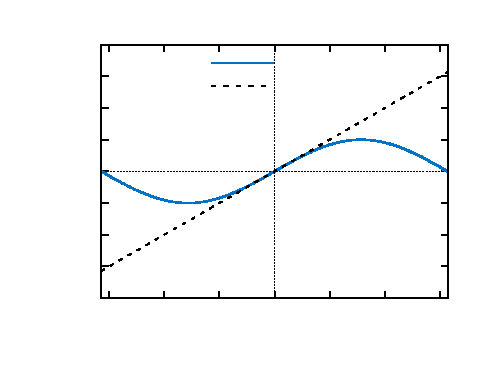
\includegraphics{sindxglobal}}%
    \gplfronttext
  \end{picture}%
\endgroup
}
 \subfloat[][]{% GNUPLOT: LaTeX picture with Postscript
\begingroup
\footnotesize
  \makeatletter
  \providecommand\color[2][]{%
    \GenericError{(gnuplot) \space\space\space\@spaces}{%
      Package color not loaded in conjunction with
      terminal option `colourtext'%
    }{See the gnuplot documentation for explanation.%
    }{Either use 'blacktext' in gnuplot or load the package
      color.sty in LaTeX.}%
    \renewcommand\color[2][]{}%
  }%
  \providecommand\includegraphics[2][]{%
    \GenericError{(gnuplot) \space\space\space\@spaces}{%
      Package graphicx or graphics not loaded%
    }{See the gnuplot documentation for explanation.%
    }{The gnuplot epslatex terminal needs graphicx.sty or graphics.sty.}%
    \renewcommand\includegraphics[2][]{}%
  }%
  \providecommand\rotatebox[2]{#2}%
  \@ifundefined{ifGPcolor}{%
    \newif\ifGPcolor
    \GPcolortrue
  }{}%
  \@ifundefined{ifGPblacktext}{%
    \newif\ifGPblacktext
    \GPblacktexttrue
  }{}%
  % define a \g@addto@macro without @ in the name:
  \let\gplgaddtomacro\g@addto@macro
  % define empty templates for all commands taking text:
  \gdef\gplbacktext{}%
  \gdef\gplfronttext{}%
  \makeatother
  \ifGPblacktext
    % no textcolor at all
    \def\colorrgb#1{}%
    \def\colorgray#1{}%
  \else
    % gray or color?
    \ifGPcolor
      \def\colorrgb#1{\color[rgb]{#1}}%
      \def\colorgray#1{\color[gray]{#1}}%
      \expandafter\def\csname LTw\endcsname{\color{white}}%
      \expandafter\def\csname LTb\endcsname{\color{black}}%
      \expandafter\def\csname LTa\endcsname{\color{black}}%
      \expandafter\def\csname LT0\endcsname{\color[rgb]{1,0,0}}%
      \expandafter\def\csname LT1\endcsname{\color[rgb]{0,1,0}}%
      \expandafter\def\csname LT2\endcsname{\color[rgb]{0,0,1}}%
      \expandafter\def\csname LT3\endcsname{\color[rgb]{1,0,1}}%
      \expandafter\def\csname LT4\endcsname{\color[rgb]{0,1,1}}%
      \expandafter\def\csname LT5\endcsname{\color[rgb]{1,1,0}}%
      \expandafter\def\csname LT6\endcsname{\color[rgb]{0,0,0}}%
      \expandafter\def\csname LT7\endcsname{\color[rgb]{1,0.3,0}}%
      \expandafter\def\csname LT8\endcsname{\color[rgb]{0.5,0.5,0.5}}%
    \else
      % gray
      \def\colorrgb#1{\color{black}}%
      \def\colorgray#1{\color[gray]{#1}}%
      \expandafter\def\csname LTw\endcsname{\color{white}}%
      \expandafter\def\csname LTb\endcsname{\color{black}}%
      \expandafter\def\csname LTa\endcsname{\color{black}}%
      \expandafter\def\csname LT0\endcsname{\color{black}}%
      \expandafter\def\csname LT1\endcsname{\color{black}}%
      \expandafter\def\csname LT2\endcsname{\color{black}}%
      \expandafter\def\csname LT3\endcsname{\color{black}}%
      \expandafter\def\csname LT4\endcsname{\color{black}}%
      \expandafter\def\csname LT5\endcsname{\color{black}}%
      \expandafter\def\csname LT6\endcsname{\color{black}}%
      \expandafter\def\csname LT7\endcsname{\color{black}}%
      \expandafter\def\csname LT8\endcsname{\color{black}}%
    \fi
  \fi
  \setlength{\unitlength}{0.0500bp}%
  \begin{picture}(4422.00,3400.00)%
    \gplgaddtomacro\gplbacktext{%
      \csname LTb\endcsname%
      \put(946,704){\makebox(0,0)[r]{\strut{}-0.3}}%
      \put(946,1109){\makebox(0,0)[r]{\strut{}-0.2}}%
      \put(946,1514){\makebox(0,0)[r]{\strut{}-0.1}}%
      \put(946,1920){\makebox(0,0)[r]{\strut{} 0}}%
      \put(946,2325){\makebox(0,0)[r]{\strut{} 0.1}}%
      \put(946,2730){\makebox(0,0)[r]{\strut{} 0.2}}%
      \put(946,3135){\makebox(0,0)[r]{\strut{} 0.3}}%
      \put(1078,484){\makebox(0,0){\strut{}-0.3}}%
      \put(1569,484){\makebox(0,0){\strut{}-0.2}}%
      \put(2060,484){\makebox(0,0){\strut{}-0.1}}%
      \put(2552,484){\makebox(0,0){\strut{} 0}}%
      \put(3043,484){\makebox(0,0){\strut{} 0.1}}%
      \put(3534,484){\makebox(0,0){\strut{} 0.2}}%
      \put(4025,484){\makebox(0,0){\strut{} 0.3}}%
      \csname LTb\endcsname%
      \put(176,1919){\rotatebox{-270}{\makebox(0,0){\strut{}$y$}}}%
      \put(2551,154){\makebox(0,0){\strut{}$x$}}%
    }%
    \gplgaddtomacro\gplfronttext{%
      \csname LTb\endcsname%
      \put(2002,2962){\makebox(0,0)[r]{\strut{}$\sin(x)$}}%
      \csname LTb\endcsname%
      \put(2002,2742){\makebox(0,0)[r]{\strut{}$x$}}%
    }%
    \gplbacktext
    \put(0,0){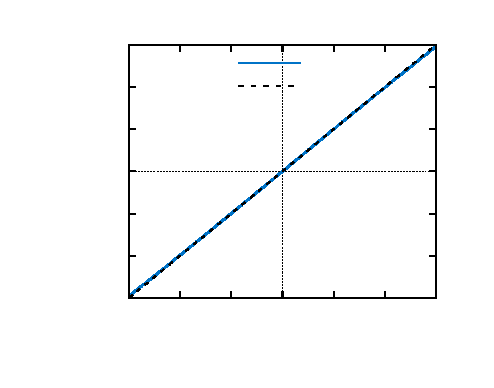
\includegraphics{sindxlocal}}%
    \gplfronttext
  \end{picture}%
\endgroup
}
 \caption[]{\quad $\sin\,\dx = \dx$: Comparing $y=\sin\,x$ and $y=x$ near $x=0$}
 \label{fig:sindx}
\end{figure}

Figure \ref{fig:sindx}(b) shows that there is virtually no difference in the
graphs even over the non-infinitesimal interval
$\ival{-0.3}{0.3}$. So $\sin\,x \approx x$ is a good approximation
when $x$ is close to 0, that is, when $\abs{x} \ll 1$ (the symbol $\ll$ means
``much less than'').\index{$\ll$} This approximation is used in many applications
in engineering and physics when the angle $x$ is assumed to be small.

Notice something else suggested by the relation $\sin\,\dx = \dx$: there is
a fundamental difference at the infinitesimal level between a line of slope 1
($y=x$) and a line of slope 0 ($y=0$). In a \emph{real} interval $(-a,a)$ around
$x=0$ the difference between the two lines can be made as small as desired by
choosing $a>0$ small enough. But in an infinitesimal interval $(-\delta,\delta)$
around $x=0$ there is unbridgeable gulf between the two lines. This is the
crucial difference in $\sin\,\dx$ being equal to $\dx$ rather than 0.

Notice also that the value of a function at an infinitesimal may itself be an
infinitesimal (e.g. $\sin\,\dx = \dx$) or a real number (e.g. $\cos\,\dx = 1$).

For a differentiable function $f(x)$, $\dfdx = f'(x)$ and so multiplying both
sides by $\dx$ yields the important relation:
\statethm{thm:df}{\vspace{-5mm}\begin{center}
 \begin{equation}\label{eqn:dffprimedx}
 \df ~=~ f'(x)\;\dx
 \end{equation}
\end{center}}
Note that both sides of the above equation are infinitesimals for each value of
$x$ in the domain of $f'$, since $f'(x)$ would then be a real number.

The notion of an infinitesimal was fairly radical at the time (and still is).
Some mathematicians embraced it, e.g. the outstanding Swiss
mathematician Leonhard Euler (1707-1783), who produced a large amount of work
using infinitesimals. But it was \emph{too} radical for
many mathematicians (and philosophers\footnote{The English philosopher George
Berkeley (1685-1753) famously derided infinitesimals as ``the ghosts of departed
quantities'' in his book \emph{The Analyst} (1734), which had the disquieting
subtitle ``A Discourse Addressed to an Infidel Mathematician'' (directed at
Newton).}), enough so
that by the 19\textsuperscript{th} century some mathematicians (notably Augustin
Cauchy and Karl Weierstrass) felt the need to put calculus on what they
considered a more ``rigorous'' footing, based on limits.\footnote{However, the
limit approach turns out, ultimately, to be equivalent to the infinitesimal
approach. In essence, only the terminology is different.}
Yet it was precisely the notion of an infinitesimal which lent calculus
its \emph{modern} character, by showing the power and usefulness of such an
abstraction (especially one that did not obey the rules of classical
mathematics).\vspace{3mm}

\divider
\vspace{3mm}
\startexercises\label{sec1dot3}
{\small
\probs{A}
\par\noindent For Exercises 1-9, let $\dx$ be an infinitesimal and prove the given formula.
\begin{enumerate}[\bfseries 1.]
\begin{multicols}{3}
 \item $(\dx \;+\; 1)^2 ~=~ 2\dx \;+\; 1$
 \item $(\dx \;+\; 1)^3 ~=~ 3\dx \;+\; 1$
 \item\label{exer:1over1plusdx} $(\dx \;+\; 1)^{-1} ~=~ 1 \;-\; \dx$
\end{multicols}
\begin{multicols}{3}
 \item $\tan\,\dx ~=~ \dx$
 \item $\sin\,2\dx ~=~ 2\dx$
 \item $\cos\,2\dx ~=~ 1$
\end{multicols}
\begin{multicols}{3}
 \item $\sin\,3\dx ~=~ 3\dx$
 \item $\cos\,3\dx ~=~ 1$
 \item $\sin\,4\dx ~=~ 4\dx$
\end{multicols}
 \item Is $\cot\,\dx$ defined for an infinitesimal $\dx$? If so, then find its value.
  If not, then explain why.
 \item In the proof of the derivative formulas for $\sin\, x$ and $\cos\, x$,
 the equation $\cos^2\,\dx = 1$ was solved to give $\cos\,\dx\ = 1$.
 Why was the other possible solution $\cos\,\dx\ = -1$ ignored?
\suspend{enumerate}
\probs{B}
\resume{enumerate}[{[\bfseries 1.]}]
 \item Show that $\ddx \,(\cos\,x) ~=~ -\sin\,x$.
 \item Show that $\ddx \,(\cos\,2x) ~=~ -2\,\sin\,2x$. \emph{(Hint: Use Exercises
 5 and 6.)}
\suspend{enumerate}
\probs{C}
\resume{enumerate}[{[\bfseries 1.]}]
 \item Show that $\ddx \,(\tan\,x) ~=~ \sec^2 \,x$. \emph{(Hint: Use Exercise 4.)}
\end{enumerate}}
\newpage
%Begin Section 1.4
\section{Derivatives of Sums, Products and Quotients}
So far the derivatives of only a few simple functions have been calculated. The
following rules will make it easier to calculate derivatives of more functions:
\index{Sum Rule}\index{Difference Rule}\index{Constant Multiple Rule}
\index{Product Rule}\index{Quotient Rule}
\index{derivative!Sum Rule}\index{derivative!Difference Rule}\index{derivative!Constant Multiple Rule}
\index{derivative!Product Rule}\index{derivative!Quotient Rule}

\statethm{thm:derivrules}{{\textbf{Rules for Derivatives:}
Suppose that $f$ and $g$ are differentiable functions of $x$. Then:
\begin{flalign*}
 \textbf{Sum Rule:}& \quad \ddx\,(f + g) ~=~ \dfdx ~+~ \dgdx &&\\[8pt]
 \textbf{Difference Rule:}& \quad \ddx\,(f - g) ~=~ \dfdx ~-~ \dgdx &&\\[8pt]
 \textbf{Constant Multiple Rule:}& \quad \ddx\,(cf) ~=~ c \cdot \dfdx \quad\text{for any constant $c$} &&\\[8pt]
 \textbf{Product Rule:}& \quad \ddx\,(f \cdot g) ~=~ f \cdot \dgdx ~+~ g \cdot \dfdx &&\\[8pt]
 \textbf{Quotient Rule:}& \quad \ddx\,\left(\dfrac{f}{g}\right) ~=~
  \dfrac{g \cdot \dfdx ~-~ f \cdot \dgdx}{g^2} &&
\end{flalign*}}}
The above rules can be written using the prime notation for derivatives:
\statethm{thm:derivrulesprime}{\vspace{-5mm}\begin{flalign*}
 \textbf{Sum Rule:}& \quad (f+g)'(x) ~=~ f'(x) ~+~ g'(x) &&\\[4pt]
 \textbf{Difference Rule:}& \quad (f-g)'(x) ~=~ f'(x) ~-~ g'(x) &&\\[4pt]
 \textbf{Constant Multiple Rule:}& \quad (cf)'(x) ~=~ c \cdot f'(x) \quad\text{for any constant $c$} &&\\[4pt]
 \textbf{Product Rule:}& \quad (f \cdot g)'(x) ~=~ f(x) \cdot g'(x) ~+~  g(x) \cdot f'(x) &&\\[4pt]
 \textbf{Quotient Rule:}& \quad \left(\dfrac{f}{g}\right)'(x) ~=~
  \dfrac{g(x) \cdot f'(x) ~-~ f(x) \cdot g'(x)}{(g(x))^2} &&
\end{flalign*}}
The proof of the Sum Rule is straightforward. Since $\dfdx$ and $\dgdx$ both exist then:
\begin{align*}
 \ddx\,(f + g) ~&=~ \dfrac{(f + g)(x + \dx) ~-~ (f + g)(x)}{\dx} ~=~
  \dfrac{f(x + \dx) ~+~ g(x + \dx) ~-~ (f(x) ~+~ g(x))}{\dx}\\[6pt]
 &=~ \dfrac{f(x + \dx) ~-~ f(x) ~+~ g(x + \dx) ~-~ g(x)}{\dx} ~=~
  \dfrac{f(x + \dx) ~-~ f(x)}{\dx} ~+~ \dfrac{g(x + \dx) ~-~ g(x)}{\dx}\\[6pt]
 &=~ \dfdx ~+~ \dgdx  \qquad \checkmark
\end{align*}
The proofs of the Difference and Constant Multiple Rules are similar and are
left as exercises.

Note that by the Product Rule, in general the derivative of a product is
\textbf{not} the product of the derivatives. That is,
$\frac{d(f \cdot g)}{\dx} \ne \dfdx \cdot \dgdx$.
This should be obvious from some earlier examples. For instance, if
$f(x) = x$ and $g(x) = 1$
then $(f \cdot g)(x) = x \cdot 1 = x$ so that $\frac{d(f \cdot g)}{\dx} = 1$,
but $\dfdx \cdot \dgdx = 1 \cdot 0 = 0$.

There is a proof of the Product Rule similar to the proof of the Sum Rule (see
Exercise 20), but there is a more geometric way of seeing why the formula holds,
described below.

\parpic[r]{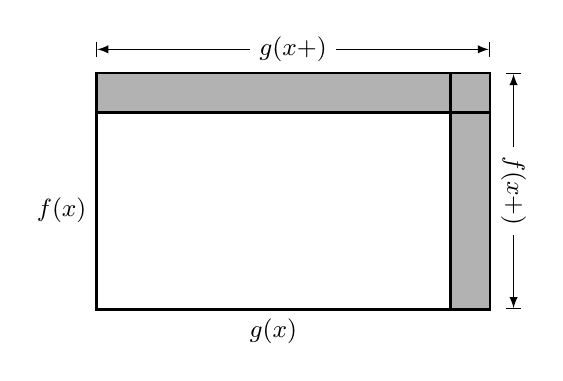
\begin{tikzpicture}[>=latex,every node/.style={font=\small}]
 \draw[|<->|] (0,3.3) -- (5,3.3);
 \node[fill=white] at (2.5,3.3) {$g(x + \dx)$};
 \draw[|<->|] (5.3,3) -- (5.3,0);
 \node[fill=white,rotate=-90] at (5.3,1.5) {$f(x + \dx)$};
 \filldraw[fill=black!30,line width=1pt] (0,0) rectangle (5,3);
 \filldraw[fill=white,line width=1pt] (0,0) rectangle (4.5,2.5);
 \draw[line width=1pt] (4.5,3) -- (4.5,2.5) -- (5,2.5);
 \node[left] at (0,1.25) {$f(x)$};
 \node[left] at (0,2.75) {$\df$};
 \node[below] at (2.25,0) {$g(x)$};
 \node[below] at (4.75,0) {$\dg$};
\end{tikzpicture}}
Construct a rectangle whose perpendicular sides have lengths $f(x)$ and $g(x)$
for some $x$, as in the drawing on the right. Change $x$ by some
infinitesimal amount $\dx$, which produces infinitesimal changes $\df$ and $\dg$
in $f(x)$ and $g(x)$, respectively. Assume those changes are positive and extend
the original rectangle by those amounts, creating a larger rectangle with
perpendicular sides $f(x + \dx)$ and $g(x + \dx)$. Then
\begin{align*}
d(f \cdot g) ~&=~ (f \cdot g)(x + \dx) ~-~ (f \cdot g)(x)\\
&=~ f(x + \dx) \cdot g(x + \dx) ~-~ f(x) \cdot g(x) &\\
&=~ \text{(area of outer rectangle)} ~-~ \text{(area of original rectangle)}\\
&=~ \text{sum of the areas of the three shaded inner rectangles}\\
&=~ f(x) \cdot \dg ~+~ g(x) \cdot \df ~+~ \df \cdot \dg\\
&=~ f(x) \cdot \dg ~+~ g(x) \cdot \df ~+~ (f'(x)\;\dx) \cdot (g'(x)\;\dx)\\
&=~ f(x) \cdot \dg ~+~ g(x) \cdot \df ~+~ (f'(x) g'(x)) \cdot (\dx)^2\\
&=~ f(x) \cdot \dg ~+~ g(x) \cdot \df ~+~ (f'(x) g'(x)) \cdot 0\\
d(f \cdot g) ~&=~  f(x) \cdot \dg ~+~ g(x) \cdot \df \quad\text{, so dividing both sides by $\dx$ yields}\\[6pt]
\frac{d(f \cdot g)}{\dx} ~&=~ f(x) \cdot \dgdx ~+~ g(x) \cdot \dfdx \quad \checkmark
\end{align*}
\picskip{0}

To prove the Quotient Rule, let $y = \frac{f}{g}$, so $f = g \cdot y$. If $y$
were a differentiable function of $x$, then the Product Rule would give
\begin{gather*}
 \dfdx ~=~ \frac{d(g \cdot y)}{\dx} ~=~ g \cdot \dydx ~+~ y \cdot \dgdx ~=~
  g \cdot \dydx ~+~ \frac{f}{g} \cdot \dgdx \quad\Rightarrow\quad
  g \cdot \dydx ~=~ \dfdx ~-~ \frac{f}{g} \cdot \dgdx\\[4pt]
 \intertext{and so dividing both sides by $g$ and getting a common denominator gives}
 \dydx ~=~ \frac{1}{g} \cdot \dfdx ~-~ \frac{f}{g^2} \cdot \dgdx ~=~
  \dfrac{g \cdot \dfdx ~-~ f \cdot \dgdx}{g^2} \quad\checkmark
\end{gather*}
A simple mnemonic device for remembering the Quotient Rule is: write
$\frac{f}{g}$ as $\frac{\text{HI}}{\text{HO}}$---so that HI represents the
``high'' (numerator) part of the quotient and HO represents the ``low''
(denominator) part---and think of $d$HI and $d$HO as the derivatives of HI and
HO, respectively. Then $\ddx\left(\frac{f}{g}\right) ~=~
\frac{\text{HO} \cdot d\text{HI} ~-~ \text{HI} \cdot d\text{HO}}{\text{HO}^2}$,
pronounced as ``ho-dee-hi minus hi-dee-ho over ho-ho.''

\begin{exmp}\label{exmp:derivtan}
 Use the Quotient Rule to show that $\ddx\,(\tan\,x) = \sec^2 x$.\vspace{1mm}
 \par\noindent\emph{Solution:} Since $\tan\,x = \frac{\sin\,x}{\cos\,x}$ then:
 \begin{align*}
  \ddx\,(\tan\,x) ~&=~ \ddx\,\left(\frac{\sin\,x}{\cos\,x}\right) ~=~
   \frac{(\cos\,x) \cdot \ddx\,(\sin\,x) ~-~ (\sin\,x) \cdot \ddx\,(\cos\,x)}{\cos^2 x} ~=~
   \frac{(\cos\,x) \cdot (\cos\,x) ~-~ (\sin\,x) \cdot (-\sin\,x)}{\cos^2 x}\\[4pt]
   &=~ \frac{\cos^2 x ~+~ \sin^2 x}{\cos^2 x} ~=~ \frac{1}{\cos^2 x} ~=~ \sec^2 x
 \end{align*}
\end{exmp}
\begin{exmp}\label{exmp:derivsec}
 Use the Quotient Rule to show that $\ddx\,(\sec\,x) = \sec\,x \; \tan\,x$.\vspace{1mm}
 \par\noindent\emph{Solution:} Since $\sec\,x = \frac{1}{\cos\,x}$ then:
 \begin{align*}
  \ddx\,(\sec\,x) ~&=~ \ddx\,\left(\frac{1}{\cos\,x}\right) ~=~
   \frac{(\cos\,x) \cdot \ddx\,(1) ~-~ 1 \cdot \ddx\,(\cos\,x)}{\cos^2 x} ~=~
   \frac{(\cos\,x) \cdot 0 ~-~ 1 \cdot (-\sin\,x)}{\cos^2 x}\\[4pt]
   &=~ \frac{\sin\,x}{\cos^2 x} ~=~ \frac{1}{\cos\,x} \cdot \frac{\sin\,x}{\cos\,x} ~=~ \sec\,x \; \tan\,x
 \end{align*}
\end{exmp}
\divider
\vspace{2mm}

Similar to the above examples, the derivatives of $\cot\,x$ and $\csc\,x$ can be
found using the Quotient Rule\index{derivative!trigonometric functions} (left as
exercises)\index{trigonometric functions}. The derivatives of all
six trigonometric functions are:

\statethm{thm:trig}{\vspace{-5mm}\begin{center}
 \begin{alignat*}{3}
  \ddx\,(\cos\,x) ~&=~ -\sin\,x \qquad\qquad\qquad& \ddx\,(\sec\,x) ~&=~ \sec\,x \; \tan\,x\\[6pt]
  \ddx\,(\sin\,x) ~&=~ \cos\,x \qquad\qquad\qquad& \ddx\,(\csc\,x) ~&=~ -\csc\,x \; \cot\,x\\[6pt]
  \ddx\,(\tan\,x) ~&=~ \sec^2 x \qquad\qquad\qquad\qquad& \ddx\,(\cot\,x) ~&=~ -\csc^2 x
 \end{alignat*}
\end{center}}

Note that the Sum and Difference Rules can be applied to sums and differences,
respectively, of not just two functions but any finite (integer) number of
functions. For example, for three differentiable functions $f_1$, $f_2$, and
$f_3$,
\begin{align*}
 \ddx\,(f_1 + f_2 + f_3) ~&=~ \frac{\df_1}{\dx} ~+~ \ddx\,(f_2 + f_3) \quad\text{by the Sum Rule}\\[4pt]
 &=~ \frac{\df_1}{\dx} ~+~ \frac{\df_2}{\dx} ~+~ \frac{\df_3}{\dx} \quad\text{by the Sum Rule again.}
\end{align*}
Continuing like this for four functions, then five functions, and so forth, the
Sum and Difference Rules combined with the Constant Multiple Rule yield the
following formula:

\statethm{thm:nsum}{For $n \ge 1$ differentiable functions $f_1$, $\ldots$, $f_n$ and
constants $c_1$, $\ldots$, $c_n$:
\begin{equation}
 \ddx\,\left(c_1 f_1 ~+~ \cdots ~+~ c_n f_n\right) ~=~
 c_1 \frac{\df_1}{\dx} ~+~ \cdots ~+~ c_n \frac{\df_n}{\dx}
\end{equation}}
Note that the above formula includes differences, by using negative
constants. The formula also shows that differentiation is a
\emph{linear operation}, which makes $\ddx$ a
\emph{linear operator}\index{linear operator}. The idea is that $\ddx$
``operates'' on differentiable functions by taking their derivatives with
respect to the variable $x$. The sum $c_1 f_1 ~+~ \cdots ~+~ c_n f_n$ is called
a \emph{linear combination} of functions, and the derivative of that linear
combination can be taken term by term, with the constant multiples taken outside
the derivatives.\index{linear combination}

A special case of the above formula is replacing the functions $f_1$, $\ldots$,
$f_n$ by nonnegative powers of $x$, making the sum a polynomial in $x$. In
previous sections the derivatives of a few polynomials---such as $x$ and
$x^2$---were calculated. For the derivative of a general
polynomial\index{derivative!Power Rule}\index{Power Rule}, the following rule is
needed:
\statethm{thm:powerrule}{
\begin{displaymath}
 \textbf{Power Rule:} \quad \ddx\,\left(x^n\right) ~=~ n\,x^{n-1} \quad\text{for any integer $n$}
\end{displaymath}}
There are several ways to prove this formula; one such way being a \textbf{proof
by induction}\index{induction}\index{proof by induction}, which in general means
using the following principle:\footnote{As Bertrand Russell noted, the name is
really a misnomer: it is actually a \emph{definition} of the natural numbers
rather than a principle, and induction technically has a different meaning.}

\statethm{thm:ind}{\textbf{Principle of Mathematical Induction}\\A statement $P(n)$
about integers $n \ge k$ is true for all $n \ge k$ if:
\begin{enumerate}
 \item $P(k)$ is true.
 \item If $P(n)$ is true for some integer $n \ge k$ then $P(n+1)$ is true.
\end{enumerate}}

The idea behind mathematical induction is simple: if a statement is true about
some initial integer $k$ (Step 1 above) and if the statement being true for
\emph{some} integer implies it is true for the \emph{next} integer (Step 2 above),
then the statement being true for $k$ implies it is true for $k+1$, which in turn
implies it is true for $k+2$, which implies it is true for $k+3$, and so forth,
making it true for \emph{all} integers $n \ge k$.

Typically the initial integer $k$ will be 0 or 1. To prove the Power Rule for
all integers, first use induction to prove the rule for all nonnegative integers
$n \ge 0$, using $k = 0$ for the initial integer. For the proof by induction,
let $P(n)$ be the statement: $\ddx\,\left(x^n\right) ~=~ n\,x^{n-1}$.
\begin{enumerate}
 \item Show that $P(0)$ is true.\\That means showing that the Power
  Rule holds for $n = 0$, i.e. $\ddx\,\left(x^0\right) ~=~ 0\,x^{0-1} = 0$.
  But $x^0 = 1$ is a constant, so its derivative is 0. $\checkmark$
 \item Assuming $P(n)$ is true for some $n \ge 0$, show that $P(n+1)$ is true.\\Assuming
 that $\ddx\,\left(x^n\right) ~=~ n\,x^{n-1}$, show that
 $\ddx\,\left(x^{n+1}\right) ~=~ (n + 1)\,x^{(n+1)-1} ~=~ (n + 1)\,x^n$. It was
 shown in Section 1.2 that $\ddx\,(x) = 1$, so:
 \begin{align*}
  \ddx\,\left(x^{n+1}\right) ~&=~ \ddx\,\left( x \cdot x^n \right)\\[4pt]
  &=~ x \cdot \ddx\,\left(x^n\right) ~+~ x^n \cdot \ddx\,\left(x\right) \quad\text{(by the Product Rule)}\\[4pt]
  &=~ x \cdot n\,x^{n-1} ~+~ x^n \cdot 1 \quad\text{(by the assumption that $P(n)$ is true)}\\[4pt]
  &=~ n\,x^n ~+~ x^n ~=~ (n + 1)\,x^n \quad\checkmark
 \end{align*}
\end{enumerate}\vspace{-5mm}
\noindent Thus, by induction, the Power Rule is true for all nonnegative
integers $n \ge 0$.

To show that the Power Rule is true for all negative integers $n < 0$, write
$n = -m$, where $m$ is positive (namely, $m = \abs{n}$). Then:
\begin{align*}
 \ddx\,\left(x^n\right) ~&=~ \ddx\,\left(x^{-m}\right) ~=~ \ddx\,\left(\frac{1}{x^m}\right) ~=~
  \frac{x^m \cdot \ddx\,(1) ~-~ 1 \cdot \ddx\,\left(x^m\right)}{\left(x^m\right)^2}
  \quad\text{(by the Quotient Rule)}\\[4pt]
 &=~ \frac{x^m \cdot 0 ~-~ 1 \cdot m\,x^{m-1}}{x^{2m}} \quad\text{(by the Power Rule for positive integers)}\\[4pt]
 &=~ -m\,x^{m-1-2m} ~=~ -m\,x^{-m-1} ~=~ n\,x^{n-1} \quad\checkmark
\end{align*}
Thus, the Power Rule is true for all integers, which completes the proof. \qedsymbol

\begin{exmp}\label{exmp:polyderiv}
 Find the derivative of $f(x) = x^4 ~-~ 4x^3 ~+~ 6x^2 ~-~ 4x ~+~ 1$.\vspace{1mm}
 \par\noindent\emph{Solution:} Differentiate the polynomial term by term and use
 the Power Rule:
 \begin{align*}
  \dfdx ~&=~ \ddx\,\left(x^4 ~-~ 4x^3 ~+~ 6x^2 ~-~ 4x ~+~ 1\right)\\[4pt]
  &=~ \ddx\,\left(x^4\right) ~-~ 4 \cdot \ddx\,\left(x^3\right) ~+~ 6 \cdot \ddx\,\left(x^2\right)
      ~-~ 4 \cdot \ddx\,\left(x\right) ~+~ \ddx\,\left(1\right)\\[4pt]
  &=~ 4x^{4-1} ~-~ 4 \cdot 3x^{3-1} ~+~ 6 \cdot 2x^{2-1} ~-~ 4 \cdot 1 ~+~ 0\\[4pt]
  &=~ 4x^3 ~-~ 12x^2 ~+~ 12x ~-~ 4
 \end{align*}
\end{exmp}
\divider
\vspace{3mm}

In general, the derivative of a polynomial of degree $n \ge 0$ is given by:
\statethm{thm:poly}{For any constants $a_0$, $\ldots$, $a_n$ with $n \ge 0$:
\begin{displaymath}
 \ddx\,\left(a_n x^n ~+~  a_{n-1} x^{n-1}\cdots ~+~ a_2 x^2 ~+~ a_1 x ~+~ a_0\right) ~=~
 n a_n x^{n-1} ~+~ (n-1)\, a_{n-1} x^{n-2} ~+~ \cdots ~+~ 2 a_2 x ~+~ a_1
\end{displaymath}}
\newpage
A way to remember the Power Rule is: bring the exponent down in front of the variable
then reduce the variable's original exponent by 1. This works even for negative exponents.

\begin{exmp}\label{exmp:polyderiv2}
 Find the derivative of $f(t) = 3t^{100} ~-~ \frac{2}{t^{100}}$.\vspace{1mm}
 \par\noindent\emph{Solution:} Differentiate term by term:
 \begin{displaymath}
  \dfdt ~=~ \ddt\,\left(3t^{100} ~-~ \frac{2}{t^{100}}\right) ~=~
             \ddt\,\left( 3t^{100} ~-~ 2t^{-100}\right)
  ~=~ 3 \cdot 100t^{99} ~-~ 2 \cdot \left(-100t^{-101}\right) ~=~ 300t^{99} ~+~ \frac{200}{t^{101}}
 \end{displaymath}
\end{exmp}
\divider
\vspace{3mm}

\startexercises\label{sec1dot4}
{\small
\probs{A}
\par\noindent For Exercises 1-14, use the rules from this section to find the
 derivative of the given function.
\begin{enumerate}[\bfseries 1.]
\begin{multicols}{2}
 \item $f(x) ~=~ x^2 ~-~ x ~-~ 1$
 \item $f(x) ~=~ x^8 ~+~ 2x^4 ~+~ 1$
\end{multicols}
\begin{multicols}{2}
 \item $f(x) ~=~ \dfrac{2x^6}{3} ~-~ \dfrac{3}{2x^6}$
 \item $f(x) ~=~ \dfrac{\sin\,x ~+~ \cos\,x}{4}\vphantom{\dfrac{2x^6}{3}}$
\end{multicols}
\begin{multicols}{2}
 \item $f(x) ~=~ x\;\sin\,x$
 \item $f(x) ~=~ x^2\;\tan\,x$
\end{multicols}
\begin{multicols}{2}
 \item $f(x) ~=~ \dfrac{\sin\,x}{x}$
 \item $f(x) ~=~ \dfrac{\sin\,x}{x^2}$
\end{multicols}
\begin{multicols}{2}
 \item $f(t) ~=~ \dfrac{2t}{1 + t^2}\vphantom{\dfrac{1 - t^2}{1 + t^2}}$
 \item $g(t) ~=~ \dfrac{1 - t^2}{1 + t^2}$
\end{multicols}
\begin{multicols}{2}
 \item $f(x) ~=~ \dfrac{ax + b}{cx + d}$ ~($a$, $b$, $c$, $d$ are constants)
 \item $F(r) ~=~ -\dfrac{G m_1 m_2}{r^2}$ ~($G$, $m_1$, $m_2$ are constants)
\end{multicols}
\begin{multicols}{2}
 \item $A(r) ~=~ \pi\,r^2\vphantom{\dfrac{4}{3}}$
 \item $V(r) ~=~ \dfrac{4}{3}\,\pi r^3$
\end{multicols}
\begin{multicols}{2}
 \item Show that $\ddx \,(\cot\,x) ~=~ -\csc^2 x$.
 \item Show that $\ddx \,(\csc\,x) ~=~ -\csc\,x \; \cot\,x$.
\end{multicols}
\suspend{enumerate}
\probs{B}
\resume{enumerate}[{[\bfseries 1.]}]
\begin{multicols}{2}
 \item Prove the Difference Rule.
 \item Prove the Constant Multiple Rule.
\end{multicols}
 \item Use the Product Rule to show that for three differentiable functions $f$,
  $g$, and $h$, the derivative of their product is
  $(fgh)' = f'gh + fg'h + fgh'$.
\suspend{enumerate}
\probs{C}
\resume{enumerate}[{[\bfseries 1.]}]
 \item Provide an alternative proof of the Product Rule for two differentiable
 functions $f$ and $g$ of $x$:
 \begin{enumerate}[\bfseries (a)]
  \item Show that $(\df)(\dg) = 0$.
  \item By definition, the derivative of the product $f \cdot g$ is
   \begin{displaymath}
    \ddx\,(f \cdot g) ~=~ \frac{f(x+\dx) \cdot g(x+\dx) ~-~ f(x) \cdot g(x)}{\dx} ~.
   \end{displaymath}
   Use that formula along with part (a) to show that
   $\ddx\,(f \cdot g) ~=~ f \cdot \dgdx ~+~ g \cdot \dfdx$.\\
   \emph{(Hint: Recall that $\df ~=~ f(x+\dx) ~-~ f(x)$.)}
 \end{enumerate}
\end{enumerate}}
\newpage
%Begin Section 1.5
\section{The Chain Rule}
From what has been discussed so far it might be tempting to think that the
derivative of a function like $\sin\,2x$ is simply
$\cos\,2x$, since the derivative of $\sin\,x$ is $\cos\,x$.
It turns out that is not correct:
\begin{align*}
 \ddx\,(\sin\,2x) ~&=~ \ddx\,(2\;\sin\,x\;\cos\,x) \quad\text{(by the double-angle formula for sine)}\\[4pt]
 &=~ 2\;\ddx\,(\sin\,x\;\cos\,x) \quad\text{(by the Constant Multiple Rule)}\\[4pt]
 &=~ 2\;\left(\sin\,x \cdot \ddx\,(\cos\,x) ~+~ \cos\,x \cdot \ddx\,(\sin\,x)\right)
     \quad\text{(by the Product Rule)}\\[4pt]
 &=~ 2\;\left(\sin\,x \cdot (-\sin\,x) ~+~ \cos\,x \cdot \cos\,x\right)\\[4pt]
 &=~ 2\;\left(\cos^2 x ~-~ \sin^2 x\right)\\[4pt]
 &=~ 2\;\cos\,2x \quad\text{(by the double-angle formula for cosine)}
\end{align*}
So the derivative of $\sin\,2x$ is $2\,\cos\,2x$, \emph{not} $\cos\,2x$.

In other words, you cannot simply replace $x$ by $2x$ in the derivative formula
for $\sin\,x$. Instead, regard $\sin\,2x$ as a \emph{composition} of
two functions: the sine function and the $2x$
function.\index{function!composition} That is, let $f(u) = \sin\,u$, where the
variable $u$ itself represents a function of another variable $x$, namely
$u(x) = 2x$. So since $f$ is a function of $u$, and $u$ is a function of $x$,
then $f$ is a function of $x$, namely: $f(x) = \sin\,2x$. Since $f$ is a
differentiable function of $u$, and $u$ is a differentiable function of $x$,
then $\dfdu$ and $\dudx$ both exist (with $\dfdu = \cos\,u$ and $\dudx = 2$),
and multiplying the derivatives shows that $f$ is a differentiable function of
$x$:
\begin{align*}
 \frac{\df}{\cancel{\du}} \cdot \frac{\cancel{\du}}{\dx} ~&=~ \dfdx
  \quad\text{since the infinitesimals $\du$ cancel, so}\\[4pt]
 (\cos\,u) \cdot 2 ~&=~ \dfdx \quad\Rightarrow\quad \dfdx ~=~ 2\;\cos\,u ~=~ 2\;\cos\,2x
\end{align*}
The above argument holds in general, and is known as the
\emph{Chain Rule}\index{derivative!Chain Rule}\index{Chain Rule}:
\statethm{thm:chainrule}{\textbf{Chain Rule:} If $f$ is a differentiable
function of $u$, and $u$ is a differentiable function of $x$, then $f$ is a
differentiable function of $x$, and its derivative with respect to $x$ is:
\begin{displaymath}
  \dfdx ~=~ \dfdu \cdot \dudx
\end{displaymath}}
Notice how simple the proof is---the infinitesimals $\du$ cancel.\footnote{Some
textbooks give dire warnings to \emph{not} think that $\du$ is an actual
quantity that can be canceled. However, you can safely ignore those warnings,
because $\du$ is just an infinitesimal and hence \emph{can} be canceled!}

The Chain Rule should make sense intuitively. For example, if $\dfdu = 4$ then
that means $f$ is increasing 4 times as fast as $u$, and if $\dudx = 3$ then $u$
is increasing 3 times as fast as $x$, so overall $f$ should be increasing
$12 = 4 \cdot 3$ times as fast as $x$, exactly as the Chain Rule says.

\begin{exmp}\label{exmp:sinx2pxp1deriv}
 Find the derivative of $f(x) = \sin\,(x^2 + x + 1)$.\vspace{1mm}
 \par\noindent\emph{Solution:} The idea is to make a \emph{substitution}
 $u = x^2 + x + 1$ so that $f(x) = \sin\,u$. By the Chain Rule,
 \begin{align*}
  \dfdx ~&=~ \dfdu \cdot \dudx\\[4pt]
  &=~ \ddu\,(\sin\,u) \;\cdot\; \ddx\,(x^2 + x + 1)\\[4pt]
  &=~ (\cos\,u) \cdot (2x + 1)\\[4pt]
  &=~ (2x + 1)\,\cos\,(x^2 + x + 1)
 \end{align*}
 after replacing $u$ by its definition as a function of $x$ in the last step;
 the final answer for the derivative should be in terms of $x$, not $u$.
\end{exmp}
\divider
\vspace{3mm}

In the Chain Rule you can think of the function in question as
the composition of an ``outer'' function $f$ and an ``inner'' function $u$;
first take the derivative of the ``outer'' function then multiply by the
derivative of the ``inner'' function. Think of the ``inner'' function as a box
into which you can put any function of $x$, and the ``outer'' function being
a function of that empty box.

For instance, for the function $f(x) = \sin\,(x^2 + x + 1)$ in the previous example,
think of the ``outer'' function as $\sin\,\Box$, where $\Box = x^2 + x + 1$ is the
``inner'' function, so that
\begin{align*}
 f(x) ~&=~ \sin\,(x^2 + x + 1)\\
 &=~ \sin\,\Box\\
 \dfdx ~&=~ \left(\cos\,\Box\right) \;\cdot\; \ddx\,\Box\\[4pt]
 &=~ \left(\cos\,\setlength{\fboxsep}{2pt}\boxed{x^2 + x + 1}\right) \;\cdot\;
     \ddx\,\setlength{\fboxsep}{2pt}\boxed{x^2 + x + 1}\\[4pt]
 &=~ (2x + 1)\,\cos\,(x^2 + x + 1)
\end{align*}

\begin{exmp}\label{exmp:chainrulepow}
 Find the derivative of $f(x) = (2x^4 - 3\cos\,x)^{10}$.\vspace{1mm}
 \par\noindent\emph{Solution:} Here the ``outer'' function is $f(\Box) = \Box^{10}$
 and the ``inner'' function is $\Box = u = 2x^4 - 3\cos\,x$:
 \begin{displaymath}
  \dfdx ~=~ \dfdu \cdot \dudx ~=~ 10\,\Box^9 \;\cdot\; \ddx\,(\Box) ~=~
             10\,(2x^4 - 3\cos\,x)^9 \;(8x^3 + 3\sin\,x)
 \end{displaymath}
\end{exmp}
\divider
\newpage
Recall that the composition $f \circ g$ of two functions $f$ and $g$ is defined
as $(f \circ g)(x) = f(g(x))$. Using prime notation the Chain Rule can be
written as: 
\statethm{thm:chainruleprime}{\textbf{Chain Rule:} If $g$ is a differentiable
function of $x$, and $f$ is a differentiable function on the range of $g$, then
$f \circ g$ is a differentiable function of $x$, and its derivative with respect
to $x$ is:
\begin{displaymath}
  (f \circ g)'(x) ~=~ f'(g(x)) \;\cdot\; g'(x)
\end{displaymath}}

Using the Chain Rule, the Power Rule can be extended to include exponents that
are rational numbers:\footnote{It will be shown in Chapter 2 how to define any
real number as an exponent. The Power Rule extends to that case as well.}
\statethm{thm:xr}{\begin{displaymath}
 \ddx\,\left(x^r\right) ~=~ r\,x^{r-1} \quad\text{for any rational number $r$}
\end{displaymath}}
% To prove this, let $y = x^r = x^{m/n} = \left(x^m\right)^{1/n}$, where $m$ and
% $n$ are integers with $n \ne 0$. Then $y^n = x^m$, so taking the derivative with
% respect to $x$ of both sides of this equation gives
To prove this, let $r = m/n$, where $m$ and $n$ are integers with $n \ne 0$.
Then $y = x^r = x^{m/n} = \left(x^m\right)^{1/n}$, so that $y^n = x^m$. Taking
the derivative with respect to $x$ of both sides of this equation gives
\begin{align*}
 \ddx\,\left(y^n\right) ~&=~ \ddx\,\left(x^m\right) \quad\text{, so evaluating the
                              left side by the Chain Rule gives}\\[4pt]
 n y^{n-1} \;\cdot\; \dydx ~&=~ m x^{m-1}\\[4pt]
 n \left(x^{m/n}\right)^{n-1} \;\cdot\; \dydx ~&=~ m x^{m-1}\\[4pt]
 \dydx ~&=~ \frac{m x^{m-1}}{n x^{m - (m/n)}} ~=~
            \frac{m}{n}\,x^{m - 1 - (m - (m/n))} ~=~ \frac{m}{n}\,x^{(m/n) - 1} ~=~
            r\,x^{r-1} \quad\checkmark
\end{align*}

\begin{exmp}\label{exmp:derivsqrtx}
 Find the derivative of $f(x) = \sqrt{x}$.\vspace{1mm}
 \par\noindent\emph{Solution:} Since $\sqrt{x} = x^{1/2}$ then by the Power
 Rule:
 \begin{displaymath}
  \dfdx ~=~ \ddx\,\left(x^{1/2}\right) ~=~ \frac{1}{2}\,x^{1/2 - 1} ~=~
            \frac{1}{2}\,x^{-1/2} ~=~
            \frac{1}{2\,\sqrt{x}}
 \end{displaymath}
\end{exmp}
\begin{exmp}\label{exmp:deriv1oversqrtx}
 Find the derivative of $f(x) = \frac{2}{3\sqrt{x}}$.\vspace{1mm}
 \par\noindent\emph{Solution:}
 \begin{displaymath}
  \dfdx ~=~ \ddx\,\left(\frac{2}{3}\,x^{-1/2}\right) ~=~
            \frac{2}{3} \cdot \frac{-1}{2}\,x^{-3/2} ~=~
            -\frac{1}{3\,x^{3/2}}
 \end{displaymath}
\end{exmp}
\divider
\vspace{3mm}
\newpage
\startexercises\label{sec1dot5}
{\small
\probs{A}
\par\noindent For Exercises 1-18, find the derivative of the given function.
\begin{enumerate}[\bfseries 1.]
\begin{multicols}{2}
 \item $f(x) ~=~ (1 ~-~ 5x)^4$
 \item $f(x) ~=~ 5\,(x^3 ~+~ x ~-~ 1)^4$
\end{multicols}
\begin{multicols}{2}
 \item $f(x) ~=~ \sqrt{1 ~-~ 2x}\vphantom{{(1-x^2)}^{\tfrac{3}{2}}}$
 \item $f(x) ~=~ (1 ~-~ x^2 )^{\tfrac{3}{2}}$
\end{multicols}
\begin{multicols}{2}
 \item $f(x) ~=~ \dfrac{\sqrt{x}}{x ~+~ 1}$
 \item $f(x) ~=~ \dfrac{\sqrt{x} ~+~ 1}{\sqrt{x} ~-~ 1}$
\end{multicols}
\begin{multicols}{2}
 \item $f(t) ~=~ \left(\dfrac{1 ~-~ t}{1 ~+~ t}\right)^4\vphantom{\left(\dfrac{x^2 ~+~ 1}{x ~-~ 1}\right)^6}$
 \item $f(x) ~=~ \left(\dfrac{x^2 ~+~ 1}{x ~-~ 1}\right)^6$
\end{multicols}
\begin{multicols}{2}
 \item $f(x) ~=~ \sin^2 x$
 \item $f(x) ~=~ \cos\,\left(\sqrt{x}\right)$
\end{multicols}
\begin{multicols}{2}
 \item $f(x) ~=~ 3 \tan\,(5x)$
 \item $f(x) ~=~ A\,\cos\,(\omega x ~+~ \phi)$ ~~($A$, $\omega$, $\phi$ are constants)
\end{multicols}
\begin{multicols}{2}
 \item $f(x) ~=~ \sec\,(x^2)\vphantom{\left(\dfrac{1}{1 - x}\right)}$
 \item $f(x) ~=~ \sin^2 \left(\dfrac{1}{1 - x}\right) ~+~ \cos^2 \left(\dfrac{1}{1 - x}\right)$
\end{multicols}
\begin{multicols}{2}
 \item $L(\beta) ~=~ \dfrac{1}{\sqrt{1 ~-~ \beta^2}}\vphantom{\left(1 ~+~ \left(\dfrac{x - l}{s}\right)^2\right)^{-1}}$
 \item $f(x) ~=~ \dfrac{1}{\pi s}\left(1 ~+~ \left(\dfrac{x - l}{s}\right)^2\right)^{-1}$
       ($s$, $l$ are constants)
\end{multicols}
\begin{multicols}{2}
 \item $f(x) ~=~ \cos\,(\cos\,x)$
 \item $f(x) ~=~ \sqrt{1 ~+~ \sqrt{x}}$
\end{multicols}
\suspend{enumerate}
\probs{B}
\resume{enumerate}[{[\bfseries 1.]}]
 \item In a certain type of electronic circuit\footnote{This is an example of a
  \emph{current-differencing negative feedback amplifier}. See pp.473-479 in
  \textsc{Schilling, D.L. and C. Belove}, \emph{Electronic Circuits: Discrete and Integrated},
  2nd ed., New York: McGraw-Hill, Inc., 1979.} the \emph{overall gain} $A_v$ is given by
  \begin{displaymath}
   A_v ~=~ \frac{A_o}{1 ~-~ T}
  \end{displaymath}
  where the \emph{loop gain} $T$ is a function of the \emph{open-loop gain} $A_o$.
  \begin{enumerate}[\bfseries (a)]
   \item Show that
    \begin{displaymath}
     \frac{d \negmedspace A_v}{d\!A_o} ~=~ \frac{1}{1 ~-~ T} ~-~ \frac{A_o}{(1 ~-~ T)^2}
                                           \frac{d \negmedspace (1 - T)}{d\!A_o} ~.
    \end{displaymath}
   \item In the case where $T$ is directly proportional to $A_o$, use part (a) to
    show that
    \begin{displaymath}
     \frac{d \negmedspace A_v}{d\!A_o} ~=~ \frac{1}{(1 ~-~ T)^2} ~.
    \end{displaymath}
    \emph{(Hint: First show that $\;A_o \cdot \frac{d \negmedspace (1 - T)}{d\!A_o} ~=~ -T$.)}
  \end{enumerate}
 \item Show that the Chain Rule can be extended to 3 functions: if $u$ is a
  differentiable function of $x$, $v$ is a differentiable function of $u$, and
  $f$ is a differentiable function of $v$, then
\begin{displaymath}
 \dfdx ~=~ \dfdv \;\cdot\; \dvdu \;\cdot\; \dudx
\end{displaymath}
so that $f$ is a differentiable function of $x$. Notice that the 3 derivatives
are linked together as in a chain (hence the name of the rule). The Chain Rule
can be extended to any finite number of functions by the above technique.
\newpage
 \item In an internal combustion engine, as a piston moves downward the connecting rod
 rotates the crank in the clockwise direction, as shown in Figure \ref{fig:crank}
below.\footnote{See pp.43-45 in \textsc{Heywood, J.B.}, \emph{Internal Combustion Engine
Fundamentals}, New York: McGraw-Hill Inc., 1988.}

 \begin{figure}[h]
 \begin{center}
  \begin{tikzpicture}[every node/.style={font=\small}]
  \draw [dashed] (0,-7.5) circle (2.5);
  \filldraw [fill=white,line width=1pt,rounded corners,rotate around={15.255:(0,0)}] (240:0.9)
   arc (240:-60:0.9) -- ([shift={(0,-5.7)}] 37.875:1.1) arc (37.875:-217.875:1.1) -- cycle;
  \filldraw [fill=white,line width=1pt,rotate around={53.13:(0,-7.5)}] (0,-6.6) -- (2.5,-6.6) arc
   (90:-90:0.9) -- (0,-8.4) arc (270:90:0.9);
  \draw[dashed] (0,0) -- (1.5,-5.5) node[black,pos=0.55,sloped,below] {connecting rod}
   node[midway,above right] {$l$};
  \draw [line width=1pt] (0,0) circle (0.6);
  \fill (0,0) circle (2pt);
  \node [above] at (0,0) {$A$};
  \draw [line width=1pt] (1.5,-5.5) circle (0.6);
  \fill (1.5,-5.5) circle (2pt);
  \node [below] at (1.5,-5.5) {$B$};
  \draw [line width=1pt] (0,-7.5) circle (0.6);
  \fill (0,-7.5) circle (2pt);
  \node [below] at (0,-7.5) {$O$};
  \draw [dashed] (0,-7.5) -- (1.5,-5.5) node[sloped,midway,below] {crank};
  \draw [dashed,latex-latex] (-2.5,-7.5) -- (-0.05,-7.5) node[pos=0.4,fill=white] {$a$};
  \draw [dashed] (0,-7.5) -- (0,0) node[pos=0.5,left] {$s$};
  \draw [dashed,-latex] (0,-6.4) arc (90:53.13:1.1);
  \node at (0.4,-6.25) {$\theta$};
  \draw [line width=1pt] (-1.3,1.2) -- (1.3,1.2) -- (1.3,-1) -- (1.7,-1) -- (1.7,2) -- (-1.7,2) --
   (-1.7,-1) -- (-1.3,-1) -- cycle;
  \node at (0,1.6) {piston};
  \pattern[pattern color=black,pattern=north east lines] (-2,2.4) -- (-1.8,2.4) -- (-1.8,-1.4)
   -- (-2,-1.4) -- cycle;
  \draw [line width=1pt] (-1.8,2.4) -- (-1.8,-1.4);
  \pattern[pattern color=black,pattern=north east lines] (2,2.4) -- (1.8,2.4) -- (1.8,-1.4)
   -- (2,-1.4) -- cycle;
  \draw [line width=1pt] (1.8,2.4) -- (1.8,-1.4);
  \draw [linecolor,line width=1.5pt,-latex] (0,2.6) -- (0,2.1);
  \draw [linecolor,line width=1.5pt,-latex] (2.7,-7.5) arc (360:330:2.7);
 \end{tikzpicture} \vspace{-5mm}
 \end{center}
 \caption[]{}
 \label{fig:crank}
\end{figure}

The point $A$ can only move vertically, causing the point $B$ to move around a circle
of radius $a$ centered at the point $O$, which is directly below the point $A$ and
does not move. As the crank rotates it makes an
angle $\theta$ with the line $\overline{OA}$. Let $l = AB$ and $s = OA$ as in
the picture. Assume that all lengths are measured in centimeters, and let the time
variable $t$ be measured in minutes.
 \begin{enumerate}[\bfseries (a)]
  \item Show that $s ~=~ a \cos\,\theta ~+~ \left(l^2 ~-~ a^2 \sin^2\theta\right)^{1/2}~$
  for $0 \le \theta \le \pi$.
  \item The \emph{mean piston speed} is $\bar{S}_p = 2LN$, where $L = 2a$ is the
   \emph{piston stroke}, and $N$ is the \emph{rotational velocity}\index{rotational velocity} of
   the crank, measured in revolutions per minute (rpm). The instantaneous piston velocity
   is $S_p = \dsdt$. Let $R = l/a$. Show that for $0 \le \theta \le \pi$,
\begin{displaymath}
 \ABS{\frac{S_p}{\bar{S}_p}} ~=~ \frac{\pi}{2}\,\sin\,\theta
 \left[1 ~+~ \frac{\cos\,\theta}{\left(R^2 - \sin^2\theta\right)^{1/2}}\right] ~~.
\end{displaymath}
 \end{enumerate}
\end{enumerate}}
\newpage
%Begin Section 1.6
\section{Higher Order Derivatives}
The derivative $f'(x)$ of a differentiable function $f(x)$ can be thought of as
a function in its own right, and if it is differentiable then its
derivative---denoted by $f''(x)$---is the
\textbf{second derivative}\index{derivative!second} of $f(x)$ (the
\textbf{first derivative}\index{derivative!first} being $f'(x)$). Likewise, the
derivative of $f''(x)$ would be the \textbf{third derivative} of $f(x)$, written
as $f'''(x)$. Continuing like this yields the fourth derivative, fifth
derivative, and so on. In general the
\textbf{$\bm{n}$-th derivative}\index{derivative!$n$-th} of $f(x)$ is
obtained by differentiating $f(x)$ a total of $n$ times. Derivatives beyond the
first are called \textbf{higher order derivatives}.\index{derivative!higher
order}\index{$f^{(n)}$}\index{$\frac{d^2y}{\dx^2}$}\index{$\frac{d^n}{\dx^n}$}

\begin{exmp}
 For $f(x) = 3x^4$ find $f''(x)$ and $f'''(x)$.\vspace{1mm}
 \par\noindent\emph{Solution:} Since $f'(x) = 12x^3$ then the second derivative
 $f''(x)$ is the derivative of $12x^3$, namely:
 \begin{displaymath}
  f''(x) ~=~ 36x^2
 \end{displaymath}
 The third derivative $f'''(x)$ is then the derivative of $36x^2$, namely:
 \begin{displaymath}
  f'''(x) ~=~ 72x
 \end{displaymath}
\end{exmp}\vspace{-2mm}
\divider
\vspace{3mm}

Since the prime notation for higher order derivatives can be cumbersome (e.g.
writing 50 prime marks for the fiftieth derivative), other notations have been
created:

\statecomment{\textbf{Notation for the second derivative of $\bm{y = f(x)}$:}
The following are all equivalent:
\begin{displaymath}
  f''(x) ~~,~~~ f^{(2)}(x) ~~,~~~ \dfrac{d^2y}{\dx^2} ~~,~~~
 \dfrac{d^2}{\dx^2}\;(f(x)) ~~,~~~  y'' ~~,~~~ y^{(2)} ~~,~~~
 \ddot{y} ~~,~~~ \ddot{f}(x) ~~,~~~ \dfrac{d^2f}{\dx^2} ~~,~~~ D^2 f(x)
\end{displaymath}
\textbf{Notation for the $\bm{n}$-th derivative of $\bm{y = f(x)}$:} The
following are all equivalent:
\begin{displaymath}
  f^{(n)}(x) ~~,~~~ \dfrac{d^ny}{\dx^n} ~~,~~~
 \dfrac{d^n}{\dx^n}\;(f(x)) ~~,~~~ y^{(n)} ~~,~~~ \dfrac{d^nf}{\dx^n} ~~,~~~ D^n f(x)
\end{displaymath}}

Notice that the parentheses around $n$ in the notation $f^{(n)}(x)$ indicate
that $n$ is not an exponent---it is the number of derivatives to take. The $n$
in the Leibniz notation $\frac{d^ny}{\dx^n}$ indicates the same thing, and in
general makes working with higher order derivatives easier:
\begin{align*}
 \frac{d^2y}{\dx^2} ~&=~ \ddx\,\left(\dydx\right)\\[4pt]
 \frac{d^3y}{\dx^3} ~&=~ \ddx\,\left(\frac{d^2y}{\dx^2}\right)
                     ~=~ \frac{d^2}{\dx^2}\,\left(\dydx\right)\\
                     &\vdots\\
 \frac{d^ny}{\dx^n} ~&=~ \ddx\,\left(\frac{d^{n-1}y}{\dx^{n-1}}\right)
                    ~=~ \frac{d^{n-1}}{\dx^{n-1}}\,\left(\dydx\right)
\end{align*}
\newpage
A natural question to ask is: what do higher order derivatives represent? Recall that
the first derivative $f'(x)$ represents the instantaneous rate of change of a function
$f(x)$ at the value $x$. So the second derivative $f''(x)$ represents the instantaneous
rate of change of the function $f'(x)$ at the value $x$. In other words, the second
derivative is a rate of change of a rate of change.

\parpic[r]{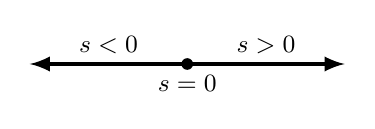
\begin{tikzpicture}[>=latex,
 every node/.style={font=\small}]
 \draw[<->,black,line width=1.5pt] (-2,0) -- (2,0) node[midway, below] {$s = 0$};
 \node[above] at (1,0) {$s > 0$}; 
 \node[above] at (-1,0) {$s < 0$}; 
 \fill (0,0) circle (2.1pt);
\end{tikzpicture}}
The most famous example of this is for motion in a straight line: let $s(t)$ be
the position of an object at time $t$ as the object moves along the line. The
motion can take two directions, e.g. forward/backward or up/down. Take one
direction to represent positive position and the other to represent negative
direction, as in the drawing on the right. The (instantaneous) velocity $v(t)$
of the object at time $t$ is $s'(t)$, i.e. the first derivative of $s(t)$. The
\textbf{acceleration}\index{acceleration} $a(t)$ of the object at time $t$ is
defined as $v'(t)$, the instantaneous rate of change of the velocity. Thus,
$a(t) = s''(t)$, i.e. acceleration is the second derivative of position. To
summarize:\index{straight line motion}

\statecomment{\vspace{-5mm}\begin{center}
\begin{align*}
 s(t) ~&=~ \text{position at time $t$}\\[4pt]
 v(t) ~&=~ \text{velocity at time $t$}\\
       &=~ \dsdt ~=~ s'(t) ~=~ \dot{s}(t)\\[6pt]
 a(t) ~&=~ \text{acceleration at time $t$}\\
       &=~ \dvdt ~=~ v'(t) ~=~ \dot{v}(t)\\[4pt]
       &=~ \ddt\,\left(\dsdt\right) ~=~ \frac{d^2s}{\dt^2} ~=~ s''(t) ~=~ \ddot{s}(t)
\end{align*}
\end{center}}

\begin{exmp}\label{exmp:accel}
 Ignoring wind and air resistance, the position $s$ of a ball thrown straight up
 with an initial velocity of 34 m/s from a starting point 2 m off the ground is
 given by $s(t) = -4.9t^2 + 34t + 2$ at time $t$ (measured in seconds) with $s$
 measured in meters.
 Find the velocity and acceleration of the ball at any time $t \ge 0$.\vspace{1mm}
 \par\noindent\emph{Solution:} The ball moves in a straight vertical line, first
 straight up then straight down until it hits the ground. Its velocity $v(t)$ is
 \begin{align*}
  v(t) ~&=~ \dsdt ~=~ -9.8t ~+~ 34 ~~\text{m/s}
 \intertext{while its acceleration $a(t)$ is}
  a(t) ~&=~ \frac{d^2s}{\dt^2} ~=~ \ddt\,\left(\dsdt\right) ~=~ \ddt\,(-9.8t ~+~ 34)
       ~=~ -9.8 ~~\text{m/s}^2\text{,}
 \end{align*}
 which is the acceleration due to the force of gravity on Earth.\\
 Note that time $t = 0$ is the time at which the ball was thrown, so that
 $v(0)$ is the initial velocity of the ball.
 Indeed, $v(0) = -9.8(0) + 34 = 34$ m/s, as expected.
\end{exmp}\vspace{-2mm}
\divider
\newpage
\parpic[r]{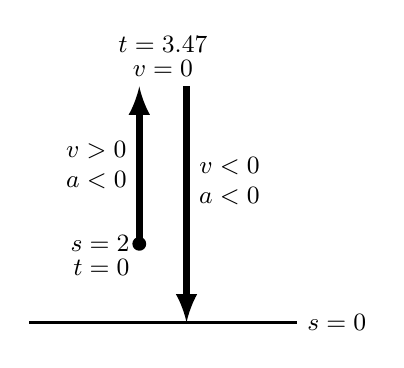
\begin{tikzpicture}[>=latex,every node/.style={font=\small}]
\draw[->,line width=2.5pt] (0,1) -- (0,3) node[midway, left, align=center] {$v > 0$\\$a < 0$};
\draw[->,line width=2.5pt] (0.6,3) -- (0.6,0) node[pos=0.4, right, align=center] {$v < 0$\\$a < 0$};
\node[above] at (0.3,3) {$v = 0$};
\node[above] at (0.3,3.3) {$t = 3.47$};
\draw[line width=1pt] (-1.4,0) -- (2,0) node[pos=1.0,right] {$s = 0$};
\node[left] at (0,1) {$s = 2$};
\node[left] at (0,0.7) {$t=0$};
\fill (0,1) circle(2.5pt);
\end{tikzpicture}}
Notice in Example \ref{exmp:accel} that the acceleration of the ball is not only
constant but also negative. To see why this makes sense, first consider the case
where the ball is moving upward. The ball has an initial upward velocity of 34
m/s then slows down to 0 m/s at the instant it reaches its maximum height above
the ground. So the velocity is decreasing, i.e. its rate of change---the
acceleration---is negative.

The ball reaches its maximum height above the ground when its velocity is zero,
that is, when $v(t) = -9.8t + 34 = 0$, i.e. at time $t = 34/9.8 = 3.47$ seconds
after being thrown (see the picture above).
The ball then starts moving downward and its velocity is
negative (e.g. at time $t = 4$ s the velocity is
$v(4) = -9.8(4) + 34 = -5.2$ m/s).
Recall that negative velocity indicates downward motion, while positive velocity
means the motion is upward (away from the Earth's center). So in the case where
the ball begins moving downward it goes from 0 m/s to a negative velocity, with
the ball moving faster towards the ground, which it hits with a velocity of
$-33.43$ m/s (why?). So again the velocity is decreasing, which again means that
the acceleration is negative.

Common terminology involving motion might cause some confusion with the above
discussion. For example, even though the ball's acceleration is negative as it
falls to the ground, it is common to say that the ball is \emph{accelerating} in
that situation, not \emph{decelerating} (as the ball is doing while moving
upward).\index{accelerating}\index{decelerating}\index{magnitude}\index{speed}
In general, \textbf{acceleration} is understood to mean that the
\textbf{magnitude} (i.e. the absolute value) of the velocity is increasing. That
magnitude is called the \textbf{speed} of the object. \textbf{Deceleration} means
the speed is decreasing.

The first and second derivatives of an object's position with respect to time
represent the object's velocity and acceleration, respectively. Do the
third, fourth, and other higher order derivatives have any physical meanings?
It turns out they do. The third derivative of position is called
the \textbf{jerk}\index{jerk} of the object. It represents the rate of change
of acceleration, and is often used in fields such as vehicle dynamics (e.g.
minimizing jerk to provide smoother braking). The fourth, fifth, and sixth
derivatives of position are called \textbf{snap}, \textbf{crackle}, and
\textbf{pop}, respectively.\footnote{Yes, those really are their names,
obviously inspired by a certain breakfast cereal. Snap has found some uses in
flight dynamics, e.g. minimizing snap to optimize flight paths of drones.}
\index{snap}\index{crackle}\index{pop}

The \textbf{zero-th derivative}\index{derivative!zero-th} $f^{(0)}(x)$ of a
function $f(x)$ is defined to be the function $f(x)$ itself:
$f^{(0)}(x) = f(x)$. There is a way to define \textbf{fractional derivatives},
e.g. the \emph{one-half derivative} $f^{(1/2)}(x)$, which will be discussed
in Chapter 6.

An immediate consequence of the definition of higher order derivatives is:
\statethm{thm:mnderiv}{\begin{center}$\dfrac{d^{m+n}}{\dx^{m+n}}\,(f(x)) ~=~
\dfrac{d^{m}}{\dx^{m}}\,\left(\dfrac{d^{n}}{\dx^{n}}\,(f(x))\right)\quad$ for
all integers $m \ge 0$ and $n \ge 0$.\end{center}}

Recall that the \textbf{factorial}\index{factorial} $n!$ of an integer $n > 0$
is the product of the integers from 1 to $n$:
\begin{displaymath}
 n! ~=~ 1 \cdot 2 \cdot 3 \cdot \;\cdots\; \cdot n
\end{displaymath}
For example:
\begin{alignat*}{3}
 1! ~&=~ 1 \qquad\qquad& 3! ~&=~ 1 \cdot 2 \cdot 3 ~=~ 6\\
 2! ~&=~ 1 \cdot 2 ~=~ 2 \qquad\qquad& 4! ~&=~ 1 \cdot 2 \cdot 3 \cdot 4 ~=~ 24
\end{alignat*}
By convention $0!$ is defined to be 1. The following statement can be proved
using induction:
\statethm{thm:nfact}{\begin{center}$\dfrac{d^n}{\dx^n}\,\left(x^n\right) ~=~ n!\quad$
for all integers $n \ge 0$\end{center}}
Thus,
\begin{displaymath}
 \dfrac{d^{n+1}}{\dx^{n+1}}\,\left(x^n\right) ~=~
 \ddx\,\left(\dfrac{d^n}{\dx^n}\,\left(x^n\right)\right) ~=~
 \ddx\,(n!) ~=~ 0
\end{displaymath}
for all integers $n \ge 0$, since $n!$ is a constant. Polynomials are linear
combinations of nonnegative powers of a variable (e.g. $x$), so the above
result combined with the Sum Rule and the Constant Multiple rule---which
also hold for higher-order derivatives---yields this important fact:
\statethm{thm:nplus1}{The $(n+1)$-st derivative (``$n$ plus first derivative'')
of a polynomial of degree $n$ is 0:\\
For any polynomial $p(x) = a_0 ~+~ a_1 x ~+~ a_2 x^2 ~+~ \cdots ~+~ a_n x^n$
of degree $n$, $\dfrac{d^{n+1}}{\dx^{n+1}}\,(p(x)) ~=~ 0$.}
This is the basis for the commonly-used statement that ``any polynomial
can be differentiated to 0'' by taking a sufficient number of derivatives. For
example, differentiating the polynomial $p(x) = 100x^{100} + 50x^{99}$ 101 times
would yield 0 (as would differentiating more than 101 times).\vspace{3mm}

\divider
\vspace{3mm}
\startexercises\label{sec1dot6}
{\small
\probs{A}
\par\noindent For Exercises 1-6 find the second derivative of the given function.
\begin{enumerate}[\bfseries 1.]
 \begin{multicols}{3}
  \item $f(x) ~=~ x^3 ~+~ x^2 ~+~ x ~+~ 1$
  \item $f(x) ~=~ x^2\,\sin x$
  \item $f(x) ~=~ \cos 3x$
 \end{multicols}
 \begin{multicols}{3}
  \item $f(x) ~=~ \dfrac{\sin x}{x}\vphantom{\dfrac{G m_1 m_2}{r^2}}$
  \item $f(x) ~=~ \dfrac{1}{x}\vphantom{\dfrac{G m_1 m_2}{r^2}}$
  \item $F(r) ~=~ \dfrac{G m_1 m_2}{r^2}$
 \end{multicols}
 \item Find the first five derivatives of $f(x) = \sin x$. Use those to find $f^{(100)}(x)$ and $f^{(2014)}(x)$.
 \item Find the first five derivatives of $f(x) = \cos x$. Use those to find $f^{(100)}(x)$ and $f^{(2014)}(x)$.
 \item If an object moves along a straight line such that its position
  $s(t)$ at time $t$ is directly proportional to $t$ for all $t$ (written as
  $s \propto t$), then show that the object's acceleration is always 0.
\suspend{enumerate}
\probs{B}
\resume{enumerate}[{[\bfseries 1.]}]
 \item\label{exer:dnxn} Use induction to show that
  $\frac{d^n}{\dx^n}\,\left(x^n\right) ~=~ n!~$ for all integers $n \ge 1$.
 \item Show that for all integers $n \ge m \ge 1$,
  $\frac{d^{m}}{\dx^{m}}\,\left(x^n\right) ~=~ \frac{n!}{(n - m)!}\,x^{n - m} ~$.
 \item Find the general expression for the $n$-th derivative of
  $f(x) = \frac{1}{ax + b} ~$ for all constants $a$ and $b$ ($a \ne 0$).
 \item Show that the function $y = A \cos\,(\omega t + \phi) ~+~  B \sin\,(\omega t + \phi)$
  satisfies the \emph{differential equation}\index{differential equation}
  \[
   \frac{d^2y}{\dt^2} ~+~ \omega^2 y ~=~ 0
  \]
  for all constants $A$, $B$, $\omega$, and $\phi$.
 \item If $s(t)$ represents the position at time $t$ of an object
 moving along a straight line, then show that:
\begin{alignat*}{2}
 s' ~\text{and}~ s'' ~&\text{have the same sign} \quad&&\Rightarrow\quad \text{the object is accelerating}\\
 s' ~\text{and}~ s'' ~&\text{have opposite signs} &&\Rightarrow\quad \text{the object is decelerating}
\end{alignat*}
 \item For all twice-differentiable functions $f$ and $g$, show that
  $\;(f \cdot g)'' = f'' \cdot g ~+~ 2 f' \cdot g' ~+~ f \cdot g''$.
\suspend{enumerate}
\probs{C}
\resume{enumerate}[{[\bfseries 1.]}]
 \item Recall that taking a derivative is a way of
 \emph{operating} on a function. That is, think of $\ddx$ as the
 \emph{differentiation operator} on the collection of differentiable functions,
 taking a function $f(x)$ to its derivative function $\dfdx$:
 \begin{center}
  \begin{tikzpicture}[every node/.style={minimum width=2cm,minimum height=8mm}]
   \path (0,0) node(a) [drop shadow,rounded corners,draw,fill=red!05] {$f(x)$}
        (5,0) node(b) [drop shadow,rounded corners,draw,fill=red!05] {$\dfdx$};
   \draw[-latex,thick] (node cs:name=a) -- (node cs:name=b) node[midway,above]
     {$\ddx$};
  \end{tikzpicture}
 \end{center}
  Likewise, $\frac{d^2}{d\!x^2}$ is an operator on twice-differentiable
  functions, taking a function $f(x)$ to its second derivative function
  $\frac{d^2 \negmedspace f}{d\!x^2}$:
 \begin{center}
  \begin{tikzpicture}[every node/.style={minimum width=2cm,minimum height=8mm}]
   \path (0,0) node(a) [drop shadow,rounded corners,draw,fill=red!05] {$f(x)$}
         (5,0) node(b) [drop shadow,rounded corners,draw,fill=red!05]
          {$\frac{d^2 \negmedspace f}{d\!x^2}$};
   \draw[-latex,thick] (node cs:name=a) -- (node cs:name=b) node[midway,above]
     {$\frac{d^2}{d\!x^2}$};
  \end{tikzpicture}
 \end{center}
  In general, an \emph{eigenfunction} of an operator $A$ is a function
  $\phi(x)$ such that $A(\phi(x)) ~=~ \lambda \cdot \phi(x)$, that is,
 \begin{center}
  \begin{tikzpicture}[every node/.style={minimum width=2cm,minimum height=8mm}]
   \path (0,0) node(a) [drop shadow,rounded corners,draw,fill=red!05]
     {$\phi(x)$} (5,0) node(b) [drop shadow,rounded corners,draw,fill=red!05]
     {$\lambda \cdot \phi(x)$};
   \draw[-latex,thick] (node cs:name=a) -- (node cs:name=b) node[midway,above]
     {$A$};
  \end{tikzpicture}
 \end{center}
  for all $x$ in the domain of $\phi$, for some constant $\lambda$ called the
  \emph{eigenvalue} of the eigenfunction.\index{eigenfunction}\index{eigenvalue}
  \begin{enumerate}[\bfseries (a)]
   \item Show for all constants $k$ that $\phi(x) ~=~ \cos\,kx$ is an
    eigenfunction of the $\frac{d^2}{d\!x^2}$ operator, and find its eigenvalue.
    That is, show that $\frac{d^2}{d\!x^2}(\phi(x)) = \lambda \cdot \phi(x)$ for
    some constant $\lambda$ (the eigenvalue).
   \item The \emph{wave function} $\psi$ for a particle of mass $m$ moving in a
    one-dimensional box of length $L$, given by
    \begin{displaymath}
     \psi(x) ~=~ \sqrt{\frac{2}{L}}\;\sin\,\frac{\pi x}{L} \qquad\text{for
     $~0 \;\le x \;\le L$,}
	\end{displaymath}
    is a solution (assuming zero potential energy) of the time-independent
    \emph{Schr\"{o}dinger equation}\index{Schr\"{o}dinger equation}
    \begin{displaymath}
     -\frac{h^2}{8\pi^2 m}\,\frac{d^2 \negmedspace\psi}{d\!x^2} ~=~ 
	 E\,\psi(x)
	\end{displaymath}
    where $h$ is \emph{Planck's constant}\index{Planck's constant}
    and $E$ is a constant that represents the total energy of the wave function.
    Find an expression for the constant $E$ in terms of the other constants.
    Notice that this makes $\psi(x)$ an
    eigenfunction of the $\frac{d^2}{d\!x^2}$ operator.
  \end{enumerate}
\end{enumerate}}
